\chapter{INTRODUCTION TO THE STANDARD MODEL}\label{Ch1}

The Particle Physics is probing the smallest objects that are known as elementary particles and tries to extend our knowledge of the subatomic world. These elementary particles are accelerated, collided and detected at very high energies in the experiments around the globe - one of them being the largest experimental setup ever built for science - and studied after being detected. \textbf{\textit{The Standard Model}} of particle physics (SM) is the theory of the fundamental interactions in this pursuit. It is a quantum field theory developed with the contribution of many scientists around the globe mainly in the second half of the 20$^{th}$ century and, over the last few decades, it has been shown to be an accurate description of the picture. It describes all known particles but is a mathematical description of three of the four known fundamental forces of the nature. These are the electromagnetic interaction, the weak and the strong nuclear interactions. The gravitational force, due to difficulties in combining general relativity with quantum mechanics, does not take place in the Standard Model. The gravity is known to be 10$^{40}$ times weaker than the electromagnetic force, thus its effects are expected to be negligible in the theory.

The Standard Model, being a quantum field theory, was formulated in the 1960's. It is grounded on the mathematical concept of the local gauge invariance under the symmetry groups of its Lagrangian equations. It has predicted successfully a wide range of phenomena which have been observed in the experiments around the globe. The discovery of the $W^\pm$ and $Z^0$ bosons at CERN's Super Proton Synchrotron (SPS) by the UA1 and UA2 Collaborations in 1983\cite{SPS-1, SPS-2, SPS-3, SPS-4, SPS-5}, the observation of the top quark at FNAL's Tevatron by D$\Phi$ and CDF Collaborations in 1995\cite{fnal-1, fnal-2}, the observation of the Higgs boson at CERN's Large Hadron Collider Experiment (LHC) by CMS and ATLAS Collaborations in 2012\cite{HiggsCMS,HiggsATLAS} and many other discoveries along with verifications can be shown as the biggest achievements of the Standard Model.

However, this successful theory had an imperfection; it could not explain the reason for the masses of the $W^\pm$ and $Z^0$ bosons. The solution came from R. Brout, F. Englert and P. Higgs in 1964 called the Brout-Englert-Higgs (BEH) Mechanism\cite{Higgs1964, BroutEnglert, Guralnik1964}. They introduced a complex scalar field into the SM and assumed a spontaneous symmetry breaking, hence giving mass to the vector bosons while preserving the unitarity of the Standard Model. This mechanism anticipated the existence of a scalar boson field. Later on, the BEH mechanism was incorporated in the electroweak model by Salam and Weingberg in 1964\cite{salam}, and proven that it is renormalisable by 't Hooft and Veltman in 1972\cite{thooft}. The predicted boson is called the Higgs boson and searched by high energy physics experiments at the forefront of scientific research nearly for 50 years.

In 1995, the technical design report for the LHC Experiment was published\cite{lhc-tdr}; it involved constructing a new particle accelerator in the Franco-Swiss border in Geneva and was intended to explore the TeV energy scale up to centre-of-mass energies of 14 TeV. This experiment has lead the front line of the experimental particle physics research for many years and discovered the Higgs boson at a mass of 125 GeV which confirmed the BEH mechanism. The details of the LHC is explained in \autoref{Ch2}.

In the SM, the elementary particles of matter and the ones that carry forces between them is grouped into two, namely fermions and bosons. The distinction shows itself in their spin properties; fermions have a spin value of half an integer whereas bosons have integer spin values. Besides, fermions obey the Pauli exclusion principle meaning that they any two fermions cannot be at the same quantum state in a bound structure, whereas bosons do not need to obey the same rule. The first generation of fermions include up and down quarks, electron and its neutrino counterpart; and bosons include photons, W and Z bosons, gluons and the Higgs boson. When added the second and the third generation of particles - whose existence is one of the mysteries of nature - along with their anti-particles, they form the fundamental particles that are known today. A tabular form of these particles can be seen in~\autoref{SM-figure}.

\vspace{6pt}
\begin{figure}[ht]
	\centering
	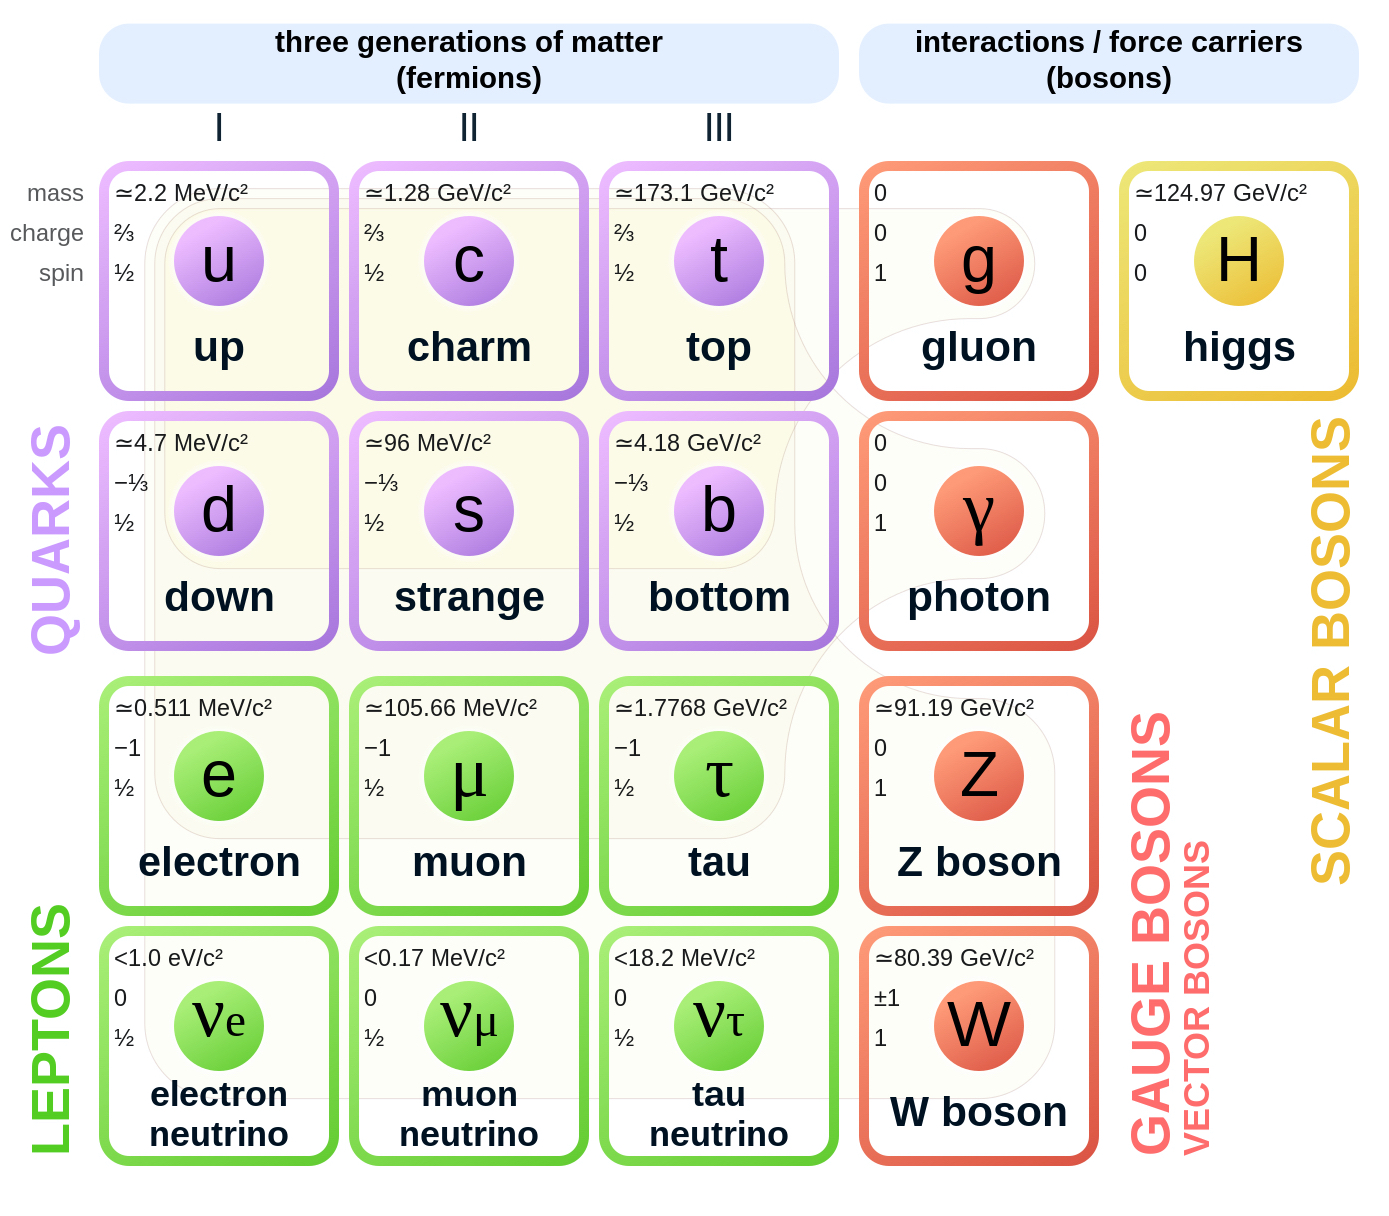
\includegraphics[width=\textwidth]{SM.jpg}
	\vspace{-0.5cm}
	\vspace{6pt}
	\caption[The elementary particles of the Standard Model. Fermions and bosons are grouped in columns where the quarks, leptons, gauge bosons and scalar Higgs boson are shown in different colours. The three generations of matter are indicated with roman numerals. The mass, charge and spin values corresponding to each particle are indicated on the upper left of each box. The vector bosons are connected in faint yellow areas to the particles they interact with.]{The elementary particles of the Standard Model. Fermions and bosons are grouped in columns where the quarks, leptons, gauge bosons and scalar Higgs boson are shown in different colours. The three generations of matter are indicated with roman numerals. The mass, charge and spin values corresponding to each particle are indicated on the upper left of each box. The vector bosons are connected in faint yellow areas to the particles they interact with \cite{SM-ref}.}
	\label{SM-figure}
\end{figure}

\textbf{Fermions} make up the ordinary matter that we see around us everyday. A subgroup of fermions are \textbf{leptons} and they include electron, muon, tau and their neutrino counterparts. Neutrinos have a very small mass compared to other leptons and quarks. They do not have electromagnetic nor colour charge which makes them obey only the weak force and they barely interact with matter. Flavours of leptons other than the neutrinos (electrons, muons and taus) have sizeable mass and charge and they are the members of the three generations of matter.

\textbf{Quarks} are the other type of fermions. They have three generations as leptons do, and they include six different flavours, namely up, down, charm, strange, top and bottom quarks. They interact with electromagnetic, weak and strong nuclear forces since they have colour charges in addition to their hypercharge. 

\textbf{Bosons} are the mediator particles of the three forces described in the SM. The particles of this type are called the gauge bosons and they include photon ($\gamma$), W$^{\pm}$ bosons, Z boson, gluons and the Higgs boson. Photons and gluons do not have mass where W bosons have about 80 GeV/c$^{2}$, Z boson 91 GeV/c$^{2}$ and the Higgs boson has 125 GeV/c$^{2}$ of mass. Among all bosons, only W$^{\pm}$ bosons have electric charge. Moreover, only the Higgs boson has a spin value of zero making it a scalar boson where all other bosons are spin-1 gauge bosons, making them vector bosons. Fermions and bosons interact with fundamental forces which we will look at now.

The \textit{\textbf{electromagnetic interaction}}, whose quantum field theory is established by the \emph{Quantum Electrodynamics (QED)}, is mediated by photons and acts only on the particles that have electric charges.  Almost everything we see in the daily life is governed by the electromagnetic force. The carrier of this force, photons, do not carry electric charge, nor self-interacts. Since photons have zero mass, their interaction range is unlimited.

The \emph{\textbf{weak nuclear force}}, which is responsible for the decay of the particles that is a flavour changing interaction, acts only on the fermions. It has a very short interaction range. The neutral and the charged current interactions are mediated by vector bosons of the this force; Z boson and W$^{\pm}$ bosons, respectively. The Higgs boson in this picture, plays the role of generating the masses of the W$^{\pm}$, and Z bosons through the Higgs mechanism~\cite{Higgs1964, BroutEnglert, Guralnik1964}, and of the quarks and leptons (except neutrinos) through Yukawa interaction\cite{Weinberg1967}.

The \textbf{\emph{Quantum Chromodynamics (QCD)}} is the theory of the \textbf{\textit{strong nuclear force}} and describes the interaction between quarks mediated by the massless gluons. It has an interaction range of about $10^{-15}$ m. Unlike the electromagnetic interaction, the gauge bosons of the strong nuclear force possess the charge of the interaction, namely colours, hence can couple to itself. There are 3 types of colour; red, green and blue and each quark in the universe carry one of these; they carry anticolour if they are antiquarks. In this fashion, gluons can be thought of colour carrier particles.

A phenomenon called the \textbf{\emph{colour confinement}} states that colour-charged particles cannot be isolated, meaning that only colour-neutral particles can be observed in nature\footnotemark. This imposes that gluons carry a pair of charge consisting a colour and an anticolour. Likewise, the hadrons are colour-neutral in two ways; i) with a pair consisting a colour and an anticolour or ii) with 3 different types of colour or anticolour. The first combination makes up mesons; consisting of a quark pair (a quark and an anti-quark), and the second combination forms baryons.

\footnotetext{~Below the Hagedorn temperature ($T_H$) of about 0.15 GeV. At the energies higher than $1.7x10^{12}$ K, hadrons become unstable and it can be thought of the boiling point of the hadronic matter~\cite{Hagedorn2016}.}

So far, we have taken a glance at the fundamental interactions and particles of the Standard Model. Many of the predictions of the Standard Model are successfully observed in the experiments, and no other particle nor force is found beyond the description given by the SM. However, the theory does not provide answer to the unsolved problems in the fundamental physics such as the non-zero masses of neutrinos\cite{neutrino-mass}, or the dark matter and the dark energy\cite{PlanckCol} which are the dominated energy content of the universe. Therefore the SM is seen as an effective field theory (EFT)\footnotemark.

\footnotetext{An effective field theory is a form of estimation for an underlying physical phenomena at a given energy or length scale. }

\section{The Standard Model Lagrangian and the Higgs Mechanism}

The Standard Model describes the behaviour of the mentioned fundamental interactions and elementary particles in a single \textbf{\textit{Lagrangian density}} formulation, often abbreviated as Lagrangian. It is often considered in two parts: the strong sector offers a description for the particles with colour charges, while the electroweak part consists of the electromagnetism and the weak force. The SM is a renormalised gauge field theory with the $ SU(3)_C \otimes SU(2)_L \otimes U(1)_Y$ gauge form and the charges are colour, weak isospin and hypercharge, respectively. The SU(2)$_L$ and U(1)$_Y$ groups mix and create the W$^{\pm}$, Z and $\gamma$ bosons where $SU(3)_C$ gauge group describes the strong force. The Lagrangian  here, does not involve the particle masses but they are introduced to the theory via the \textbf{\emph{spontaneous symmetry breaking}} (SSB) of the the electroweak gauge group $SU(2)_L \otimes U(1)_Y$, which we will address after studying the SM Lagrangian.

Mathematical interpretation of the SM is provided by the \textbf{\emph{Quantum Field Theory (QFT)}}, where each particle is represented by a quantum field that is pervaded across the space-time. Most of the field theories normally starts with defining a set of symmetries of the system and continues with writing down the renormalisable Lagrangian of the particles or fields that obey these symmetries. The QFT also follows this path; it consists of translational symmetry, rotational symmetry and a boost symmetry that is the invariance of an inertial reference frame. Under these symmetries, the Lagrangian of the SM can be interpreted in three parts; Quantum Chromodynamics, Electroweak theory and the Higgs Mechanism.

\subsection{Quantum Chromodynamics}

Starting from the free-field Dirac Lagrangian density for a massless spin-1/2 fermion, which is the quark field in the QCD case, reads,
\be
\Lag=\bar\psi\left(x\right)\left(i\gamma^\mu\partial_\mu\right)\psi(x) \; ,
\ee
where $\psi$ is the free-field for the fermion and $\gamma^\mu$ represents the Dirac matrices. The explanation below is valid with a mass term of $m\bar\psi\psi$, and $\cancel{\partial}_\mu \equiv \partial_\mu\gamma^\mu \equiv \partial^\mu\gamma_\mu$ is implied. The reason to discuss massless fermions is explained in the next two sections. The transformation of the fermion field under the $SU(3)_C$ group reads,
\be
\psi(x)\rightarrow e^{ig\frac{\lambda^a}{2}\theta_a(x)}\psi(x) \; ,
\ee
where $\frac{\lambda^a}{2}$ are the 8 Gell-Mann matrices and generators of the group. It is worth noting that $\partial_\mu\psi(x)$ does not transform in the same way and needs a redefinition, such that,
\be
D_\mu=\partial_\mu-igA_\mu^a(x)\frac{\lambda^a}{2} \; ,
\ee
where the gauge vector fields $A_\mu^a$ represent the eight gluons. These gluon fields must transform in a specific way to satisfy the local gauge invariance, such that,
\be
A_\mu^a \rightarrow A_\mu^a+\partial_\mu\theta^a+gf^{abc}A_\mu^c\theta^c \; ,
\ee
where $f^{abc}$ denotes the structure constants according to the following commutation $\left[ \frac{\lambda^a}{2}, \frac{\lambda^b}{2} \right] = if^{abc}\frac{\lambda^c}{2}$. We have achieved the invariance of the Lagrangian density by introducing the vector fields. Lastly, adding the kinetic term, whose form is
\be
-\frac{1}{4}F_a^{\mu\nu}F_{\mu\nu}^a \; ,
\ee
where
\be
F_{\mu\nu}^a=\partial_\mu A_\nu^a-\partial_\nu A_\mu^a+gf^{abc}A_\mu^bA_\nu^c \; .
\label{qcd-kinetic-term}
\ee
The complete QCD Lagrangian density becomes,
\be
\Lag_{QCD} = \bar\psi\left(i\gamma^\mu\partial_\mu\right)\psi(x)-g\bar\psi(x)\gamma^\mu\frac{\lambda_a}{2}\psi(x)A_\mu^a-\frac{1}{4}F_a^{\mu\nu}F_{\mu\nu}^a \; ,
\label{qcd-lag}
\ee

where a summation convention is implied over all of the quark fields. In the Lagrangian density, the first term is the same free-field propagation as in the original equation and the second term emerges from the interaction of the quark field with the introduced vector field $A_\mu$ along with the covariant derivative. The constant $g$ parametrises the interaction strength and is usually redefined as $\alpha_s=g^2/4\pi$ which is the strong coupling constant. The third term in the \autoref{qcd-kinetic-term}, when substituted in \autoref{qcd-lag} in the kinetic term, results in the cubic and quartic self coupling of the gluon fields which are a general feature of the non-Abelian gauge theories. The gluons and the quark fields are produced via imposing the local gauge invariance, and $SU(3)_C$ group provides the 8 generators that are the 8 gluons of the strong force.

\subsection{Electroweak theory}

Electroweak interactions are explained with the same local gauge invariance but under the $SU(2)_L\otimes U(1)_Y$ group. The parity violating nature of the weak interactions requires defining different interactions for fermions of opposite chiralities. The left hand chirality projection operator is defined as $\frac{1-\gamma^5}{2}$ where the corresponding operator for the right hand chirality projection is $\frac{1+\gamma^5}{2}$, where $\gamma^5$ is defined as
\be
\gamma^5\equiv\gamma^0\gamma^1\gamma^2\gamma^3 \; ;
\ee
and for a massless particle, the chirality corresponds to the helicity of that particle which is the normalised projection of the spin vector on the momentum vector.

The first part of the symmetry group, $SU(2)_L$, is associated with the weak isospin ($I$), and is a non-Abelian gauge group. The gauge invariance under the $SU(2)_L$ group introduces $W_\mu^i$, the gauge fields where i runs over the three generators of this group. Fermion fields are stated with chirality components as left-handed doublets and right-handed singlets, and right handed particles do not interact with the $W_\mu^i$ gauge fields.

The second part, $U(1)_Y$ is an Abelian group. $B_\mu$ is the gauge field of this group, associated with weak hypercharge ($Y$) and results from the local gauge invariance. This field interacts with both the left and right handed particles. Here, the weak hypercharge symmetry is defined different than the Quantum Electrodynamics (QED) in order to unify the electrodynamics with the weak interactions. The relation between the electric charge Q and the hypercharge $Y_W$ is given by the Gell-Mann-Nishjima formula;
\be
Q = I_3 + \frac{1}{2}Y_W \; ,
\label{hypercharge}
\ee
where $I_3$ is the third component of the weak isospin. The fermion fields can now be written as one doublet $\psi_L$ field and, two singlet $\psi_R$ and $\psi\prime_R$ fields, such that,
\be
\psi_L = \frac{1-\gamma^5}{2}
\begin{pmatrix}
    \psi \\
    \psi\prime
\end{pmatrix}
= \begin{pmatrix}
    \psi_L \\
    \psi\prime_L
\end{pmatrix} \; ,
\ee
\be
\psi_R=\frac{1+\gamma^5}{2}
\begin{pmatrix}
    \psi \\
    \psi\prime
\end{pmatrix}
= \begin{pmatrix}
    \psi_R \\
    \psi\prime_R
\end{pmatrix} \; ,
\ee
where $\psi$ and $\psi\prime$ denotes either neutrino, charged lepton fields or up, down-type quark fields. A leptoquark coupling is not predicted in the SM nor observed, meaning that these two sectors are separate. In other words, these two sectors cannot transform lepton fields into quark fields, vice-versa.

The Lagrangian density so far, consists of 3 main parts,
\be
\begin{aligned}
\Lag &= \Lag_{kin} + \Lag_{CC} + \Lag_{NC}\\
 &= i\bar\psi_L\cancel{D}\psi_L+i\bar\psi_R\cancel{D}\psi_R+i\bar\psi\prime_R\cancel{D}\psi\prime_R \; ,
\end{aligned}
\ee
where
\be
D_\mu = \partial_\mu-igW_\mu^iT_i-ig\prime\frac{Y_\psi}{2}B^\mu \; ,
\ee
and $T_i=\frac{\sigma_i}{2}$ which represents the Pauli matrices that are the generators of the $SU(2)_L$ group with eigenvalues that are actually the weak isospin values. $\Lag_{CC/NC}$ formalism here corresponds to the charged-current and neutral-current interactions, respectively. The Lagrangian density can then be rewritten as,
\be
\Lag_{kin} = i\bar\psi_L\cancel{\partial}\psi_L+i\bar\psi_R\cancel{\partial}\psi_R+i\bar\psi\prime_R\cancel{\partial}\psi\prime_R \; ,
\ee

\be
\begin{aligned}
\Lag_{CC} &= gW_\mu^1\bar\psi_L\gamma^\mu\frac{\sigma_1}{2}\psi_L+gW_\mu^2\bar\psi_L\gamma^\mu\frac{\sigma_2}{2}\psi_L\\
 &= \frac{g}{\sqrt{2}}W_\mu^+\bar\psi_L\gamma^\mu\sigma^+\psi_L+\frac{g}{\sqrt{2}}W_\mu^-\bar\psi_L\gamma^\mu\sigma^-\psi_L \; ,
\end{aligned}
\ee

\be
\begin{aligned}
\Lag_{NC} &= \frac{g}{\sqrt{2}}W_\mu^3
\left(\bar\psi_L\gamma_\mu\psi_L
-\bar\psi\prime_L\gamma_\mu\psi\prime_L\right)
+\frac{g\prime}{2}B_\mu
[Y_{\psi_L}\left(\bar\psi_L\gamma^\mu\psi_L
+\bar\psi\prime_L\gamma^\mu\psi\prime_L\right)\\
& +Y_{\psi_R}\left(\bar\psi_R\gamma^\mu\psi_R\right)Y_{\psi\prime_L}\left(\bar\psi\prime_R\gamma^\mu\psi\prime_R\right)] \; ,
\end{aligned}
\label{NClag}
\ee
where
\be
W_\mu^\pm = \frac{1}{\sqrt{2}}\left(W_\mu^1\mp iW_\mu^2\right)\sigma_\mu^\pm = \frac{1}{2}\left(\sigma^1\pm i\sigma^2\right) \; ,
\ee
which is the charged current interaction between the $\psi_L$ and $\psi\prime_L$ fields mediated by charged weak boson with $W_\mu^\pm$ fields. The neutral current field is described by the neutral Z boson field $Z_\mu$ and the photon field $A_\mu$. This interactions could not be mediated by the $W_\mu^3$ field nor by $B_\mu$, since both couples to neutral fields. The relation between these fields are given by,
\be
B_\mu = A_\mu cos\theta_W-Z_\mu sin\theta_W \; ,
\label{Z1}
\ee
\be
W_\mu^3 = A_\mu sin\theta_W + Z_\mu cos\theta_W \; ,
\label{Z2}
\ee
where $\theta_W$ is the Weinberg angle. The neutral current interactions are derived by substituting \autoref{Z1} and \autoref{Z2} in \autoref{NClag}, resulting in the coupling strength of $gsin\theta_WI_3+g\prime cos\theta_W\frac{Y}{2}$ for $A_\mu$  field. The electroweak unification is achieved by equating this coupling strength to the photon field's coupling constant. Since the hypercharge is only multiplied by $g\prime$, we can set an arbitrary value for it as $Y_{\psi_L} = -1$. This process then gives, along with $Q = -1$ for leptons and 0 for neutrinos,
\be
gsin\theta_W = g\prime cos\theta_W = e \; ,
\ee
The Lagrangian density for the electroweak interactions then becomes,
\be
\Lag_{EW} = i\bar\psi_L\cancel{D}\psi_L+i\bar\psi_R\cancel{D}\psi_R+\bar\psi\prime_R\cancel{D}\psi\prime_R-\frac{1}{4}B_{\mu\nu}B^{\mu\nu}-\frac{1}{4}W_{\mu\nu}^iW_i^{\mu\nu} \; ,
\label{EWLag}
\ee
where
\be
B_{\mu\nu} = \partial_\mu B_\nu-\partial_\nu B_\mu \; ,
\ee
\be
W_{\mu\nu}^i = \partial_\mu W_{\nu}^i-\partial_\nu W_{\mu}^i + g\epsilon^{abc}W_\mu^bW_\nu^c \; ,
\ee

\autoref{EWLag} includes the charged and neutral interactions of fermions. Expanding the kinetic terms of the weak bosonic field yields the self couplings of the gauge bosons including the trilinear and quartic couplings. The mass terms for the bosonic fields violates the local gauge invariance as the same is valid for the strong force. Also, they are not allowed for the fermionic fields since the left and right chiralities transform individually which we will see in the next section. A list of fermionic fields is shown in \autoref{fermionfieldstable}.

\begin{table*}[ht]
	{\setlength{\tabcolsep}{14pt}
		\caption{Fermion fields under $SU(2)_L$ group representation.}
		\begin{center}
			\vspace{-6mm}
			\scalebox{0.78}{
			\begin{tabular}{cccccccc}
				\hline \\[-2.45ex] \hline \\[-2.1ex]
				Type & $1^{st}$ gen. & $2^{nd}$ gen. & $3^{rd}$ gen. & $I_3$ & $Y$ & $Q$ & $SU(3)_C$ \\
				\hline \\[-1.8ex]
				 & $\begin{pmatrix} u_L \\ d_L \end{pmatrix}$ & $\begin{pmatrix} c_L \\ s_L \end{pmatrix}$ & $\begin{pmatrix} t_L \\ b_L \end{pmatrix}$ & $\begin{pmatrix} 1/2 \\ -1/2 \end{pmatrix}$ & 1/3 & $\begin{pmatrix} 2/3 \\ -1/3 \end{pmatrix}$ & \\
				 Quarks & $u_R$ & $c_R$ & $t_R$ & 0 & 4/3 & 2/3 & triplet\\
				 & $d_R$ & $s_R$ & $b_R$ & 0 & -2/3 & -1/3 &\\
                \hline \\[-1.8ex]
				 & $\begin{pmatrix} \nu_{e,L} \\ e_L  \end{pmatrix}$ & $\begin{pmatrix} \nu_{\mu,L} \\ \mu_L \end{pmatrix}$ & $\begin{pmatrix} \nu_{\tau,L} \\ \tau_L \end{pmatrix}$ & $\begin{pmatrix} 1/2 \\ -1/2 \end{pmatrix}$ & -1 & $\begin{pmatrix} 0 \\ -1 \end{pmatrix}$ & \\
				 Leptons & $e_R$ & $\mu_R$ & $\tau_R$ & 0 & -2 & 1 & singlet \\
				\hline
			\end{tabular}}
			\vspace{-6mm}
		\end{center}
		\label{fermionfieldstable}}
\end{table*}

In brief, the fermion fields share the same composition; the left and right chirality fields are doublet and singlets under the $SU(2)_L$ group, respectively, resulting in the possession of the weak isospin in the doublets. This interaction is mediated by the $W^\pm$ bosons where neutral interactions is mediated by the Z boson; it interacts with both chiralities but this time with a different coupling strength due to the mixing of the gauge fields shown in \autoref{Z1} and \autoref{Z2}. The electromagnetic interaction is mediated by photons that is only sensitive to electric charge Q, hence to hypercharge Y and to weak isospin $I_3$ with the relation given in \autoref{hypercharge}.

The interactions between fields may differ the quantum numbers by carrying charges; the strong interactions can change the colour charge of quarks, and charged weak interactions can change the weak isospin, hence the electric charge of fermions. The Standard Model concept, explaining the matter fields by quantum numbers and the interactions by symmetry applications is an elegant mathematical theory, however the experimentally observed massive $W^\pm$ and Z bosons requires an addition to the theory, explained in the next section.

\subsection{Higgs mechanism}\label{higgsmechanismsection}

So far, we have built the SM on the assumption that the interactions are gauge invariant. This requires the vector bosons $W^\pm$ and $Z$ to be massless. In addition, for a fermion field $\psi$ satisfying the Dirac equation $ (i\hbar\gamma^\mu\partial_\mu-mc)\psi = 0$, the mass term $-m\bar\psi\psi$ arises which is actually not invariant under the $SU(2)_L$ gauge symmetry. This can be seen by expanding the mass term with left and right handed fermion fields, that is
\be
-m\bar\psi\psi = -m\left(\bar\psi_L\psi_R + \bar\psi_R\psi_L\right) ,
\ee
and we have seen that the left-handed fields are doublets under $SU(2)_L$ while right-handed fields are singlet. This means that their gauge quantum numbers are different and this kind of mass term is forbidden. 
The solution to these theoretically massless but experimentally massive particles is given by \textbf{\emph{the Brout-Englert-Higgs (BEH) Mechanism}}~\cite{Higgs1964, BroutEnglert, Guralnik1964}, usually called the Higgs Mechanism, showing that the electroweak symmetry can be broken spontaneously under specific conditions. 

The solution starts with introducing a complex scalar field $\phi$ to the theory, which is a doublet under $SU_L(2)$,
\be
 \phi = 
 \begin{pmatrix}
  \phi_+ \\
  \phi_0
 \end{pmatrix} ,
\ee\\
This field has a hypercharge value $Y=1$ and the corresponding covariant derivative,
\be
D_\mu = \partial_\mu-igW_\mu^i\frac{\sigma_i}{2}-\frac{1}{2}ig\prime B_\mu \; .
\label{higgscovariantD}
\ee
The Lagrangian describing the Higgs field becomes,
\be
 \Lag_{Higgs} = \left(D_\mu\phi\right)^\dagger\left(D^\mu\phi\right)-V\left(\phi^\dagger\phi\right) \; .
 \label{HiggsLag}
\ee

Since the potential $V$ must satisfy SU(2) and U(1) symmetries, a good solution is a Mexican hat potential;
\be
 V(\phi) = -\mu^2\phi^\dagger\phi + \lambda\left(\phi^\dagger\phi\right)^2 \; .
 \label{higgspotential}
\ee
A spontaneous symmetry breaking happens when both the constants $\mu^2$ and $\lambda$ are positive values. A convenient choice for the minimum would be
\be
\langle\phi\rangle=\frac{1}{\sqrt{2}}
 \begin{pmatrix}
  0 \\
  v
 \end{pmatrix} \; .
\ee
The minimum of this potential is non-zero with the potential shape in \autoref{mexicanHiggs} and given by,
\be
 \begin{aligned}
 \frac{dV}{d\left(\phi^\dagger\phi\right)} &=\mu^2+2\lambda\phi^\dagger\phi = 0 \\
 & \Rightarrow |\phi_{min}| = \sqrt{\frac{\mu^2}{2\lambda}} \equiv \frac{v^2}{2} \; ,
 \end{aligned}
\ee
where $v$ is called the \textbf{\emph{vacuum expectation value}} (vev). The symmetry is broken once a particular ground state is chosen but the Lagrangian density remains gauge invariant. 
\vspace{6pt}
\begin{figure}[ht]
	\centering
	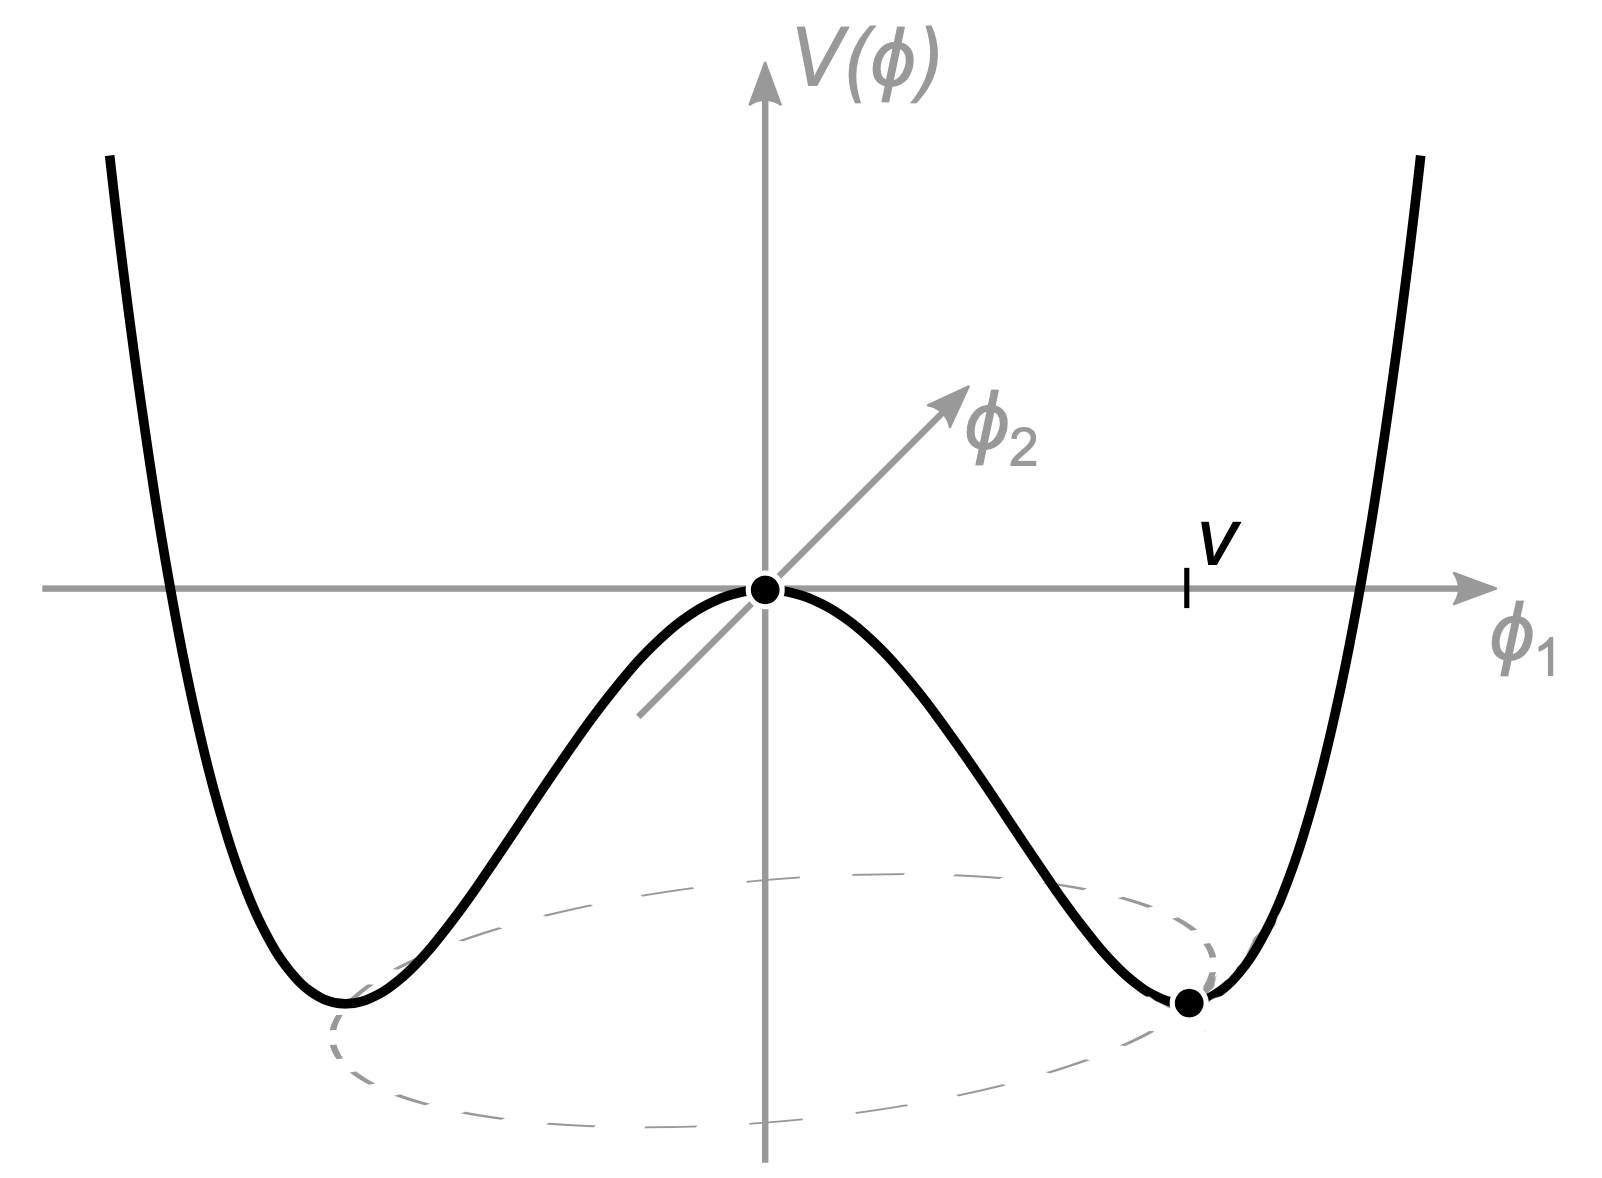
\includegraphics[scale=0.4]{mexicanhat.png}
	\vspace{-0.25cm}
	\vspace{6pt}
	\caption{The Higgs potential V in the case that $\mu^2 > 0$. Choosing any point at the bottom of the potential breaks spontaneously the rotational U(1) symmetry.}
	\label{mexicanHiggs}
\end{figure}
Now let us expand the complex doublet field around the minimum $\phi(x)$,
\be
\langle\phi\rangle=\frac{1}{\sqrt{2}}e^{\frac{i\sigma_i\theta^i(x)}{v}}
 \begin{pmatrix}
  0 \\
  v+h(x)
 \end{pmatrix} .
 \label{higgsVparametrized}
\ee
This corresponds to a real scalar massive field, to three massless \textbf{\textit{Goldstone boson fields}} $\theta^i$, which are not observed in nature. These  bosons may be created as many as the broken generators and can be removed with an $SU(2)_L$ transformation with a unitary gauge choice:
\be
\phi(x)\rightarrow\phi\prime(x)=e^{-\frac{i\sigma_i\theta^i(x)}{v}}\phi(x)=\frac{1}{\sqrt{2}}
 \begin{pmatrix}
    0 \\
    v+h(x)
 \end{pmatrix} \; .
 \label{Higgsunitarygauge}
\ee
This transformation yields only the real scalar field. Substituting \autoref{higgscovariantD} and \autoref{Higgsunitarygauge}, the Lagrangian density with the Higgs field $h$, becomes
\be
\begin{aligned}
\Lag_{Higgs} &= \frac{1}{2}\partial^\mu h\partial_\mu h-\frac{1}{2}\left(2\lambda v^2\right)h^2\\
 & + \left[\left(\frac{gv}{2}\right)^2W^{\mu +}W_\mu^- +\frac{1}{2}\frac{\left(g^2+g\prime^2\right)v^2}{4}Z^\mu Z_\mu \right]\left(1+\frac{h}{v}\right)^2\\
 & -\lambda vh^3-\frac{\lambda}{4}h^4+\frac{\lambda}{4}v^4 \; .
\end{aligned}
\ee

The first two terms represent the kinetics of the Higgs field with the mass value $m_H^2 = 2\lambda v^2=2\mu^2$. The third term represents the weak boson masses with these values;
\be
m_W^2=\frac{g^2v^2}{4} \Rightarrow m_W = \frac{gv}{2} \; ,
\ee
\be
m_Z^2 = \frac{\left(g^2+g\prime^2\right)v^2}{4}=\frac{m_W^2}{cos^2\theta_W} \Rightarrow m_Z = \frac{m_W}{cos\theta_W} \; .
\ee
It can bee seen that the removed Goldstone bosons returned as extra degrees of freedom for the $W^\pm$ and $Z$ bosons. The weak bosons gained mass via this mechanism. The third term of the Lagrangian defines the interactions between the Higgs and the weak bosons. It can be seen that the contributions of $H-WW/ZZ$ interactions come from $2h/v$ term and of $HH-WW/ZZ$ interactions from $h
^2/v^2$ term when the square bracket is expanded. The final terms demonstrate the cubic and quartic self-couplings of the Higgs field.
The potential now can be rewritten with the self-couplings as,
\be
V(h) = \frac{1}{2}m_h^2h^2+\lambda_{hhh}vh^3+\frac{1}{4}\lambda_{4h}h^4-\frac{\lambda}{4}v^4 \; ,
\ee
where the self interaction couplings are defined as,
\be
\lambda_{hhh}=\lambda_{4h}=\frac{m_h^2}{2v^2} \; .
\ee

Here, it is worth noting that these two self-couplings are  depended on the Higgs boson mass and the vacuum expectation value. Their experimental measurement provides a practical test for the SM and the electroweak symmetry breaking. There is one last term in the Higgs potential, $ -\lambda v^4/4$. This constant, being irrelevant in the SM, contributes to the cosmological constant and is not compatible with the astronomical observations\cite{Sol2013}. This is another mystery yet to be solved in the SM.

There is now the mass of the Higgs boson and the vacuum expectation value as free parameters to SM. The vacuum expectation value can be calculated precisely with the muon lifetime \cite{griffiths2008introduction}, such that,
\be
\frac{G_F}{\sqrt{2}} = \left(\frac{g}{2\sqrt{2}}\right)^2\frac{1}{m_W^2} \Rightarrow v = \sqrt{\frac{1}{\sqrt{2}G_F}} \approx 246 GeV \; ,
\ee
where $G_F$ is the Fermi constant.
Mass terms for the fermions are generated by the Higgs field's Yukawa interaction between the left and right chiral fields. The interaction's Lagrangian density can be written as,
\be
\Lag_{Yukawa} = -y_{f\prime}\left(\bar\psi_L\phi\psi\prime_R+\bar\psi\prime_R\phi^\dagger\psi_L\right)
- y_f\left(\bar\psi_L\tilde\phi\psi_R+\bar\psi_R\tilde\phi^\dagger\psi_L\right) \; ,
\ee
with the broken symmetry,
\be
\tilde\phi = i\sigma_2\phi^* = \begin{pmatrix} \phi_0^* \\ -\phi_+^* \end{pmatrix} \xRightarrow[\text{}]{\text{EWSB}} \frac{1}{\sqrt{2}} \begin{pmatrix} v+h(x)\\ 0 \end{pmatrix} \; ,
\ee
where $\psi$ denotes up and $\psi\prime$ denotes down-type fermions. When the \textbf{\textit{Electroweak Symmetry Breaking (EWSB)}} applied, the Lagrangian density reads,
\be
\Lag_{Yukawa} = -\sum_f m_f\left(\bar\psi_L\psi_R+\bar\psi_R\psi_L\right)\left(1+\frac{h}{v}\right) \; ,
\ee
where up and down-type fermions are summed with the mass terms,
\be
m_f\prime = y_f\prime\frac{v}{\sqrt{2}} \; .
\ee
No we have given the explanation for the fermion masses generated via the interaction with the Higgs field. The strengths of the interactions depend on the fermion masses; stronger interactions with heavier particles.

Finally the Standard Model Lagrangian becomes,
\be
\begin{aligned}
\Lag_{SM} &= -\frac{1}{4}F_{\mu\nu}F^{\mu\nu}-\frac{1}{4}W_{\mu\nu}W^{\mu\nu}-\frac{1}{4}B_{\mu\nu}B^{\mu\nu}\\
 & +\bar\psi i\gamma^\lambda D_\lambda \psi + \left(D_\mu\phi\right)^\dagger\left(D^\mu\phi\right)-V\left(\phi^\dagger\phi\right)\\
 & + \Lag_{Yukawa}+ h.c. \; .
\end{aligned}
\ee
The EWSB is shown later to be a renormalisable theory 't Hooft and Veltman \cite{thooft}.

The Higgs boson, required for the spontaneous symmetry breaking, was found experimentally by the CMS and ATLAS Experiments at the LHC Experiment at CERN\cite{HiggsCMS,HiggsATLAS} in 2012, almost 50 years after its theoretical assumption. The mass of the Higgs boson is 125 GeV and its parameters; spin, parity and branching ratios are found to be consistent with the Standard Model predictions\cite{Higgsprecision1, Higgsprecision2}.

The most general form of the SM Lagrangian depends on 19 parameters. These parameters are given in \autoref{SMparameters}.
\begin{table*}[ht]
	{\setlength{\tabcolsep}{14pt}
		\caption{Free parameters of the Standard Model.}
		\begin{center}
			\vspace{-6mm}
			\begin{tabular}{cccc}
				\hline \\[-2.45ex] \hline \\[-2.1ex]
				\# & Symbol & Name & Value \\
				\hline \\[-1.8ex]
				1 & $m_e$ & Electron mass & 0.511 MeV \\
				2 & $m_\mu$ & Muon mass & 105.7 MeV \\
				3 & $m_\tau$ & Tau mass & 1.78 GeV \\
				4 & $m_u$ & Up quark mass & 1.9 MeV \\
				5 & $m_d$ & Down quark mass & 4.4 MeV \\
				6 & $m_s$ & Strange quark mass & 87 MeV \\
				7 & $m_c$ & Charm quark mass & 1.32 GeV \\
				8 & $m_b$ & Bottom quark mass & 4.24 GeV \\
				9 & $m_t$ & Top quark mass & 173.5 GeV \\
				10 & $\theta_{12}$ & CKM 1-2 Mixing angle & 13.1\textdegree \\
				11 & $\theta_{23}$ & CKM 2-3 Mixing angle & 2.4\textdegree \\
				12 & $\theta_{13}$ & CKM 1-3 Mixing angle & 0.2\textdegree \\
				13 & $\delta$ & CKM CP violation Phase & 0.995 \\
				14 & $g_1$ or $g\prime$ & U(1) gauge coupling & 0.357 \\
				15 & $g_2$ or g & SU(2) gauge coupling & 0.652 \\
				16 & $g_3$ or $g_s$ & SU(3) gauge coupling & 1.221 \\
				17 & $\theta_{QCD}$ & QCD vacuum angle & $\sim $ 0 \\
				18 & $v$ & Higgs vacuum expectation value & 246 GeV \\
				19 & $m_H$ & Higgs mass & 125 GeV \\
				\hline
			\end{tabular}
			\vspace{-6mm}
		\end{center}
		\label{SMparameters}}
\end{table*}

\section{The Higgs Boson Phenomenology and Experimental Status}\label{higgs-status}

The Higgs boson, with its zero spin, is different from any other particle in the Standard Model. It does not carry any electric or colour charge hence does not take part in the electromagnetic and strong interactions. Nonetheless, it interacts with fermions and heavy bosons including itself, since it carries weak isospin. The coupling strengths of the Higgs boson to those particles are derived in \autoref{higgsmechanismsection}. These couplings are only dependent on the masses of the particles which Higgs couple to, resulting in stronger coupling strengths to heavier particles.

The discovery of the Higgs Boson in 2012 was made with the data collected at the Run-1 of the CMS and ATLAS Detectors at $\sqrt{s} = 7$ and $8$ TeV with an integrated luminosity of about $5 fb^{-1}$ in its decays to $H\rightarrow bb$, $H\rightarrow ZZ$, $H\rightarrow \gamma\gamma$, $H\rightarrow WW$ and $H\rightarrow \tau\tau$. Further data at $\sqrt{s} = 13$ TeV collected with the same detectors at Run-2 confirmed the discovery, shown in \autoref{higgs-13tev}. The mass of the Higgs boson is given by the Particle Data Group\cite{pdg} as, $ m_H = 125.25\pm 0.17$, and a summary of the mass measurements resulting to this value is shown in \autoref{higgsmasssummary}. The Higgs boson was also shown to have a spin-parity, $J^P=0^+$ \cite{higgs-spin}. The results of the Higgs boson searches showed good agreements with the Standard Model predictions.

\begin{figure*}[ht]
        \centering
        \begin{subfigure}[b]{0.475\textwidth}
            \centering
            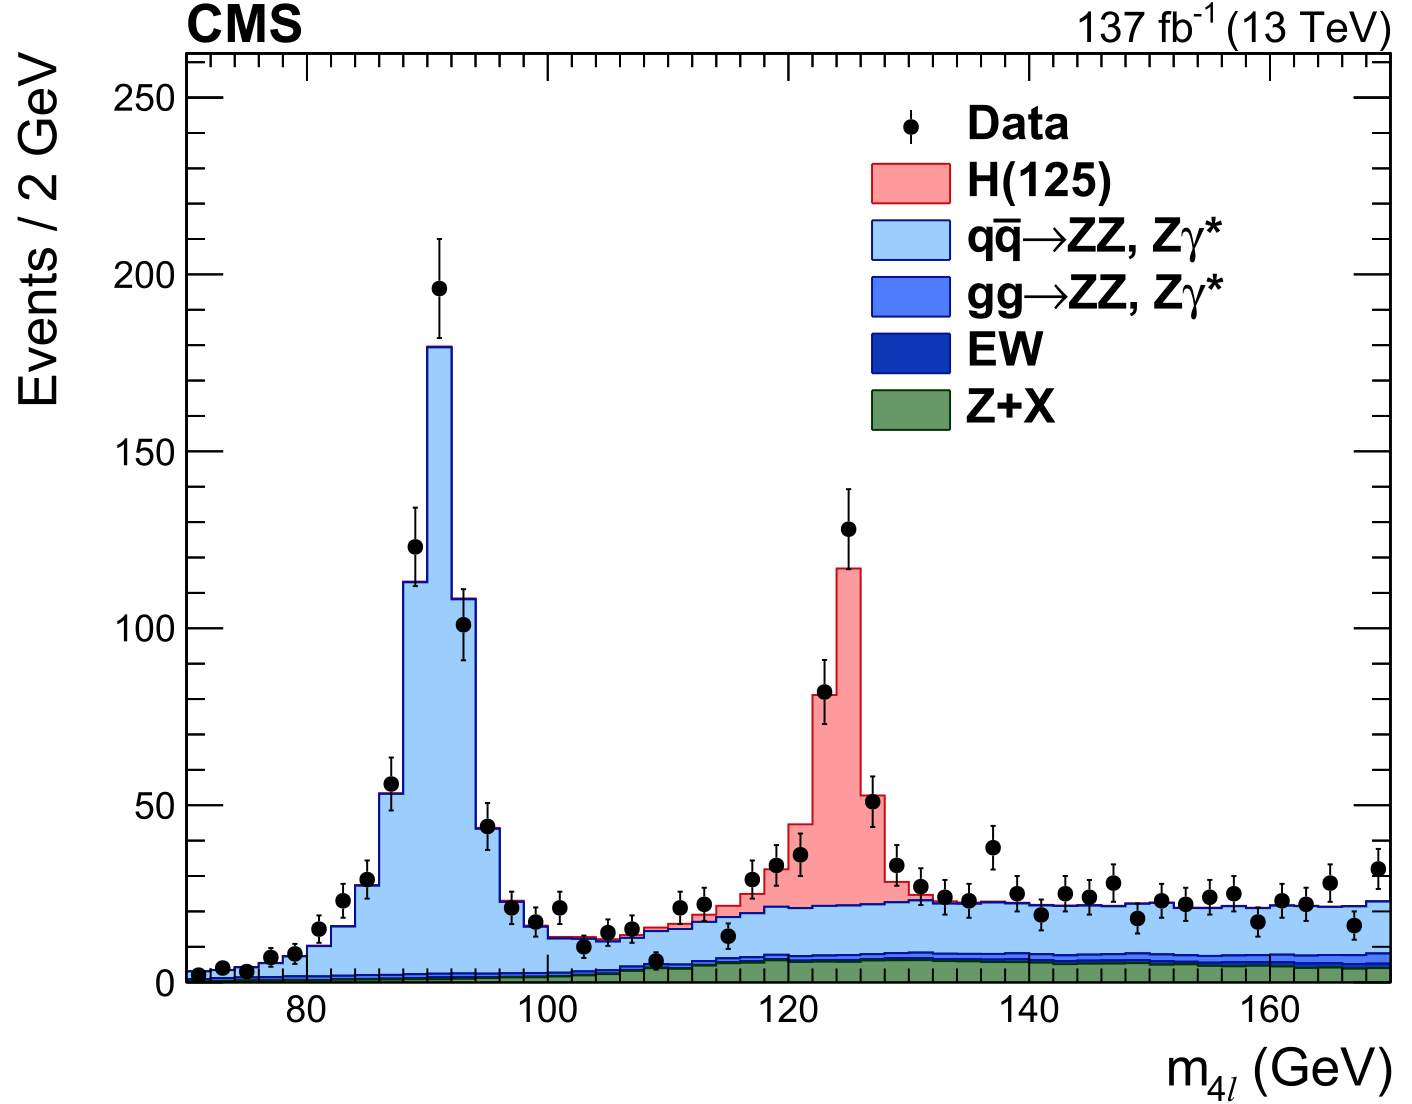
\includegraphics[width=\textwidth]{cms-higgs-13tev.png}
            \vspace{-0.5cm}
            \firstsubcaption{$m_{4l}$}
        \end{subfigure}
        \hspace{0.2cm}
        \begin{subfigure}[b]{0.475\textwidth}  
            \centering 
            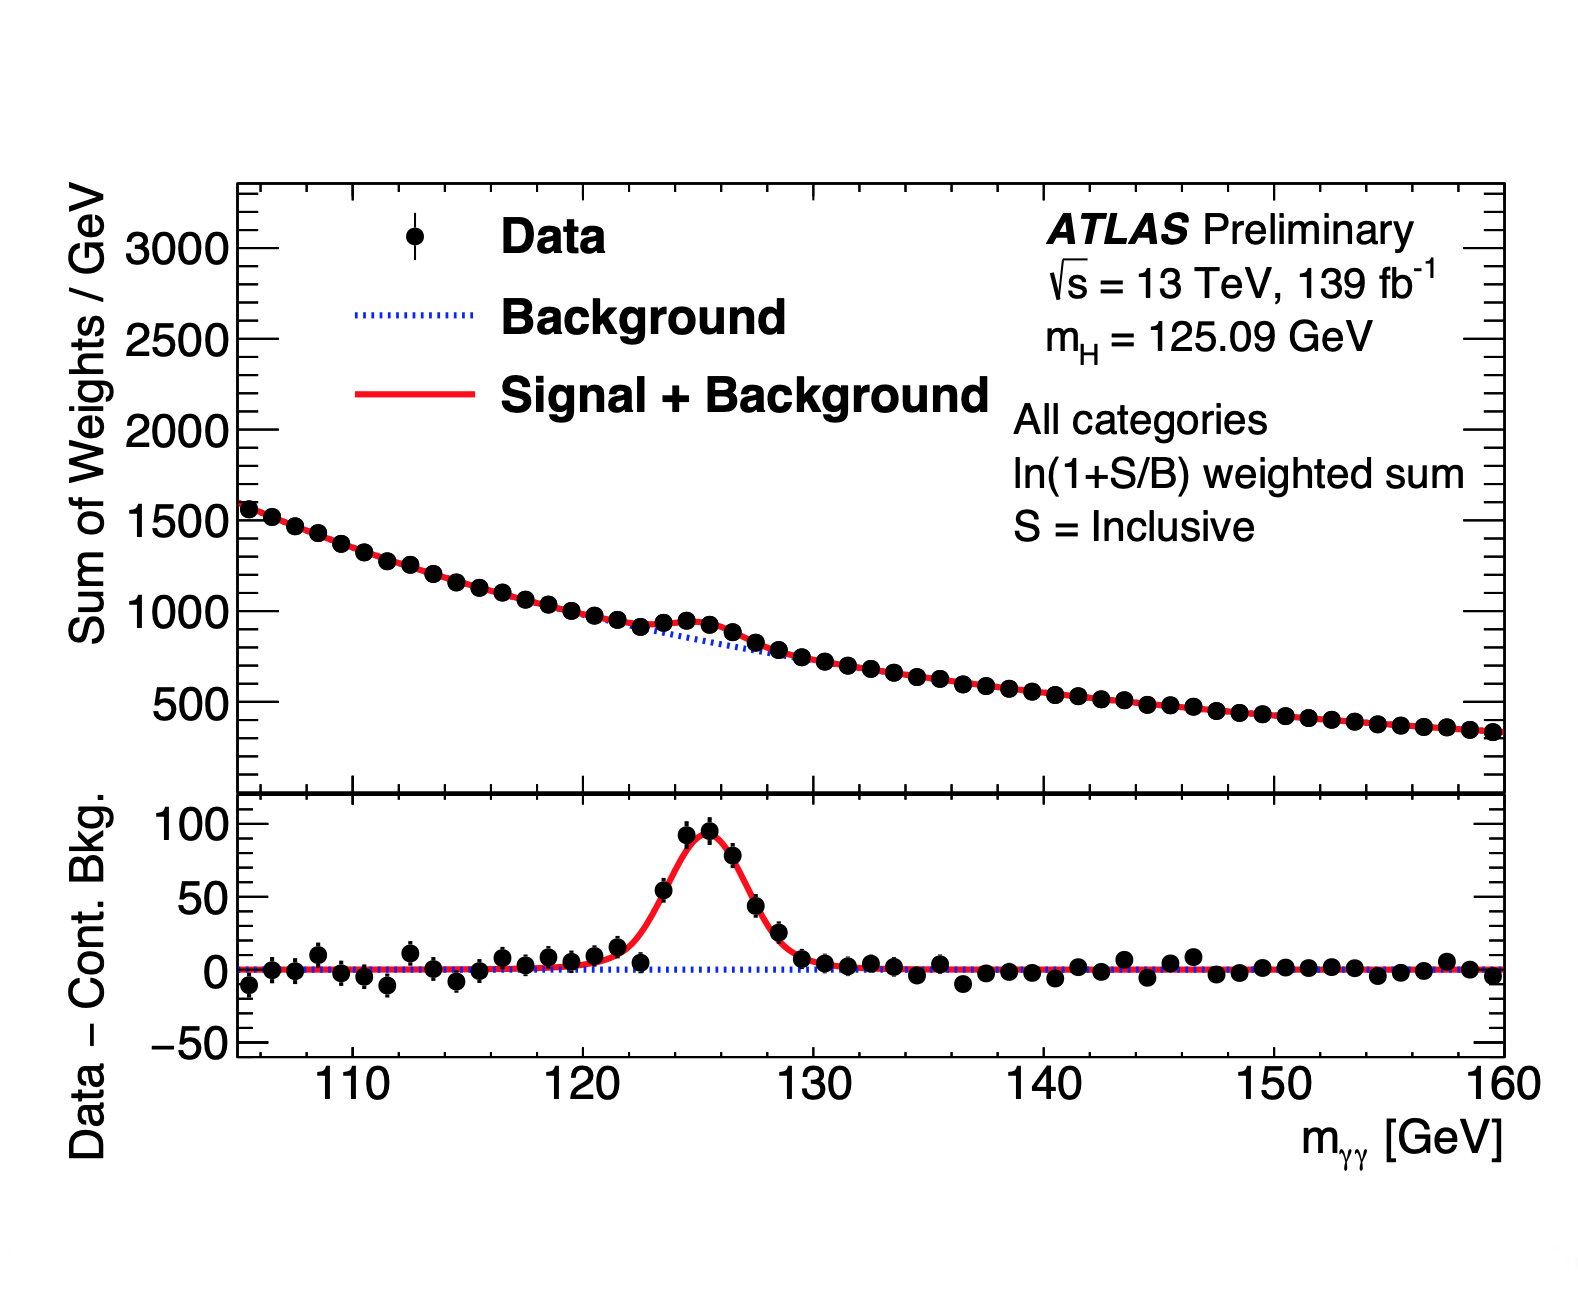
\includegraphics[width=\textwidth]{atlas-higgs-13tev.png}
            \vspace{-0.5cm}
            \firstsubcaption{$m_{\gamma\gamma}$}
        \end{subfigure}
        \caption[Four-lepton mass distribution, $m_{4l}$ obtained from the data collected at the CMS Detector on the left, and diphoton invariant mass distribution obtained from the data collected at the ATLAS Detector on the right, both at $\sqrt{s}=13$ TeV in Run II.]
        {\small Four-lepton mass distribution, $m_{4l}$ obtained from the data collected at the CMS Detector\cite{cms-higgs-13tev} on the left, and diphoton invariant mass distribution obtained from the data collected at the ATLAS Detector\cite{atlas-higgs-13tev} on the right, both at $\sqrt{s}=13$ TeV in Run II.} 
        \label{higgs-13tev}
\end{figure*}

\begin{figure}[ht]
	\centering
	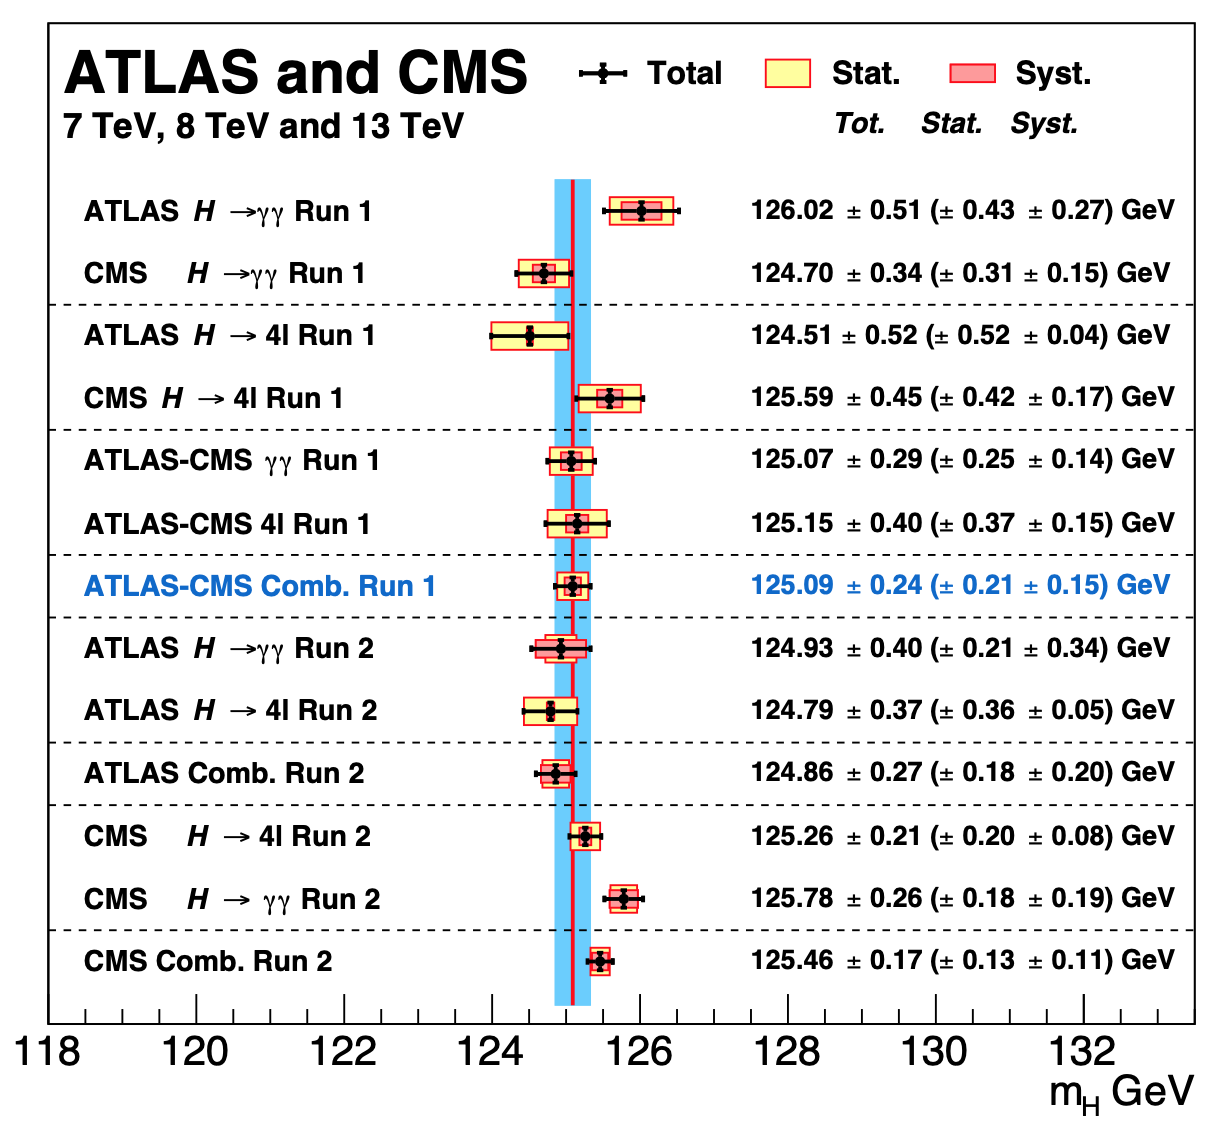
\includegraphics[scale=0.55]{higgsmasscombined.png}
	\caption[Summary of the CMS and ATLAS Higgs mass measurements in the $\gamma\gamma$ and $ZZ$ channels in Run I and Run II.]{Summary of the CMS and ATLAS Higgs mass measurements in the $\gamma\gamma$ and $ZZ$ channels in Run I and Run II\cite{pdg}.}
	\label{higgsmasssummary}
\end{figure}

The phenomenology of the Higgs boson at the LHC (the LHC is explained in \autoref{Ch2}), has been thoroughly studied \cite{higg-phen-1,higg-phen-2,higg-phen-3}. Four main production modes of the Higgs boson at the hadron colliders have been discovered. The Feynman diagrams corresponding to these production mechanism are shown in \autoref{HiggsFeynman}, and the cross sections at the proton-proton (pp) collisions at the LHC is shown in \autoref{HiggsxsecTable} in 4 different production mechanism. The production modes other than these four have very small cross sections.

\begin{table*}[ht]
	{\setlength{\tabcolsep}{14pt}
		\caption[Cross section (in pb) of the Higgs boson production at different centre-of-mass ($\sqrt{s}$) energies for $m_H=125$ GeV. The theoretical uncertainties can be found in the reference.]{Cross section (in pb) of the Higgs boson production at different centre-of-mass ($\sqrt{s}$) energies for $m_H=125$ GeV. The theoretical uncertainties can be found in \cite{pdg}.}
		\begin{center}
			\vspace{-6mm}
			\begin{tabular}{cccccc}
				\hline \\[-2.45ex] \hline \\[-2.1ex]
				$\sqrt{s}$ (TeV) &&&Production mode&&\\
				\hline \\[-1.8ex]
				& $ggF$ & $VBF$ & $VH$ & $t\bar tH$ & Total \\
				\hline \\[-1.8ex]
                1.96 & 0.95 & 0.065 & 0.209 & 0.004 & 1.23 \\
                7 & 16.9 & 1.24 & 0.92 & 0.09 & 19.1 \\
                8 & 21.4 & 1.60 & 1.12 & 0.13 & 24.2 \\
                13 & 48.6 & 3.78 & 2.25 & 0.5 & 55.1 \\
                14 & 54.7 & 4.28 & 2.5 & 0.61 & 62.1 \\
				\hline
			\end{tabular}
			\vspace{-6mm}
		\end{center}
		\label{HiggsxsecTable}}
\end{table*}

\begin{figure*}[ht]
        \centering
        \begin{subfigure}[b]{0.475\textwidth}
            \centering
            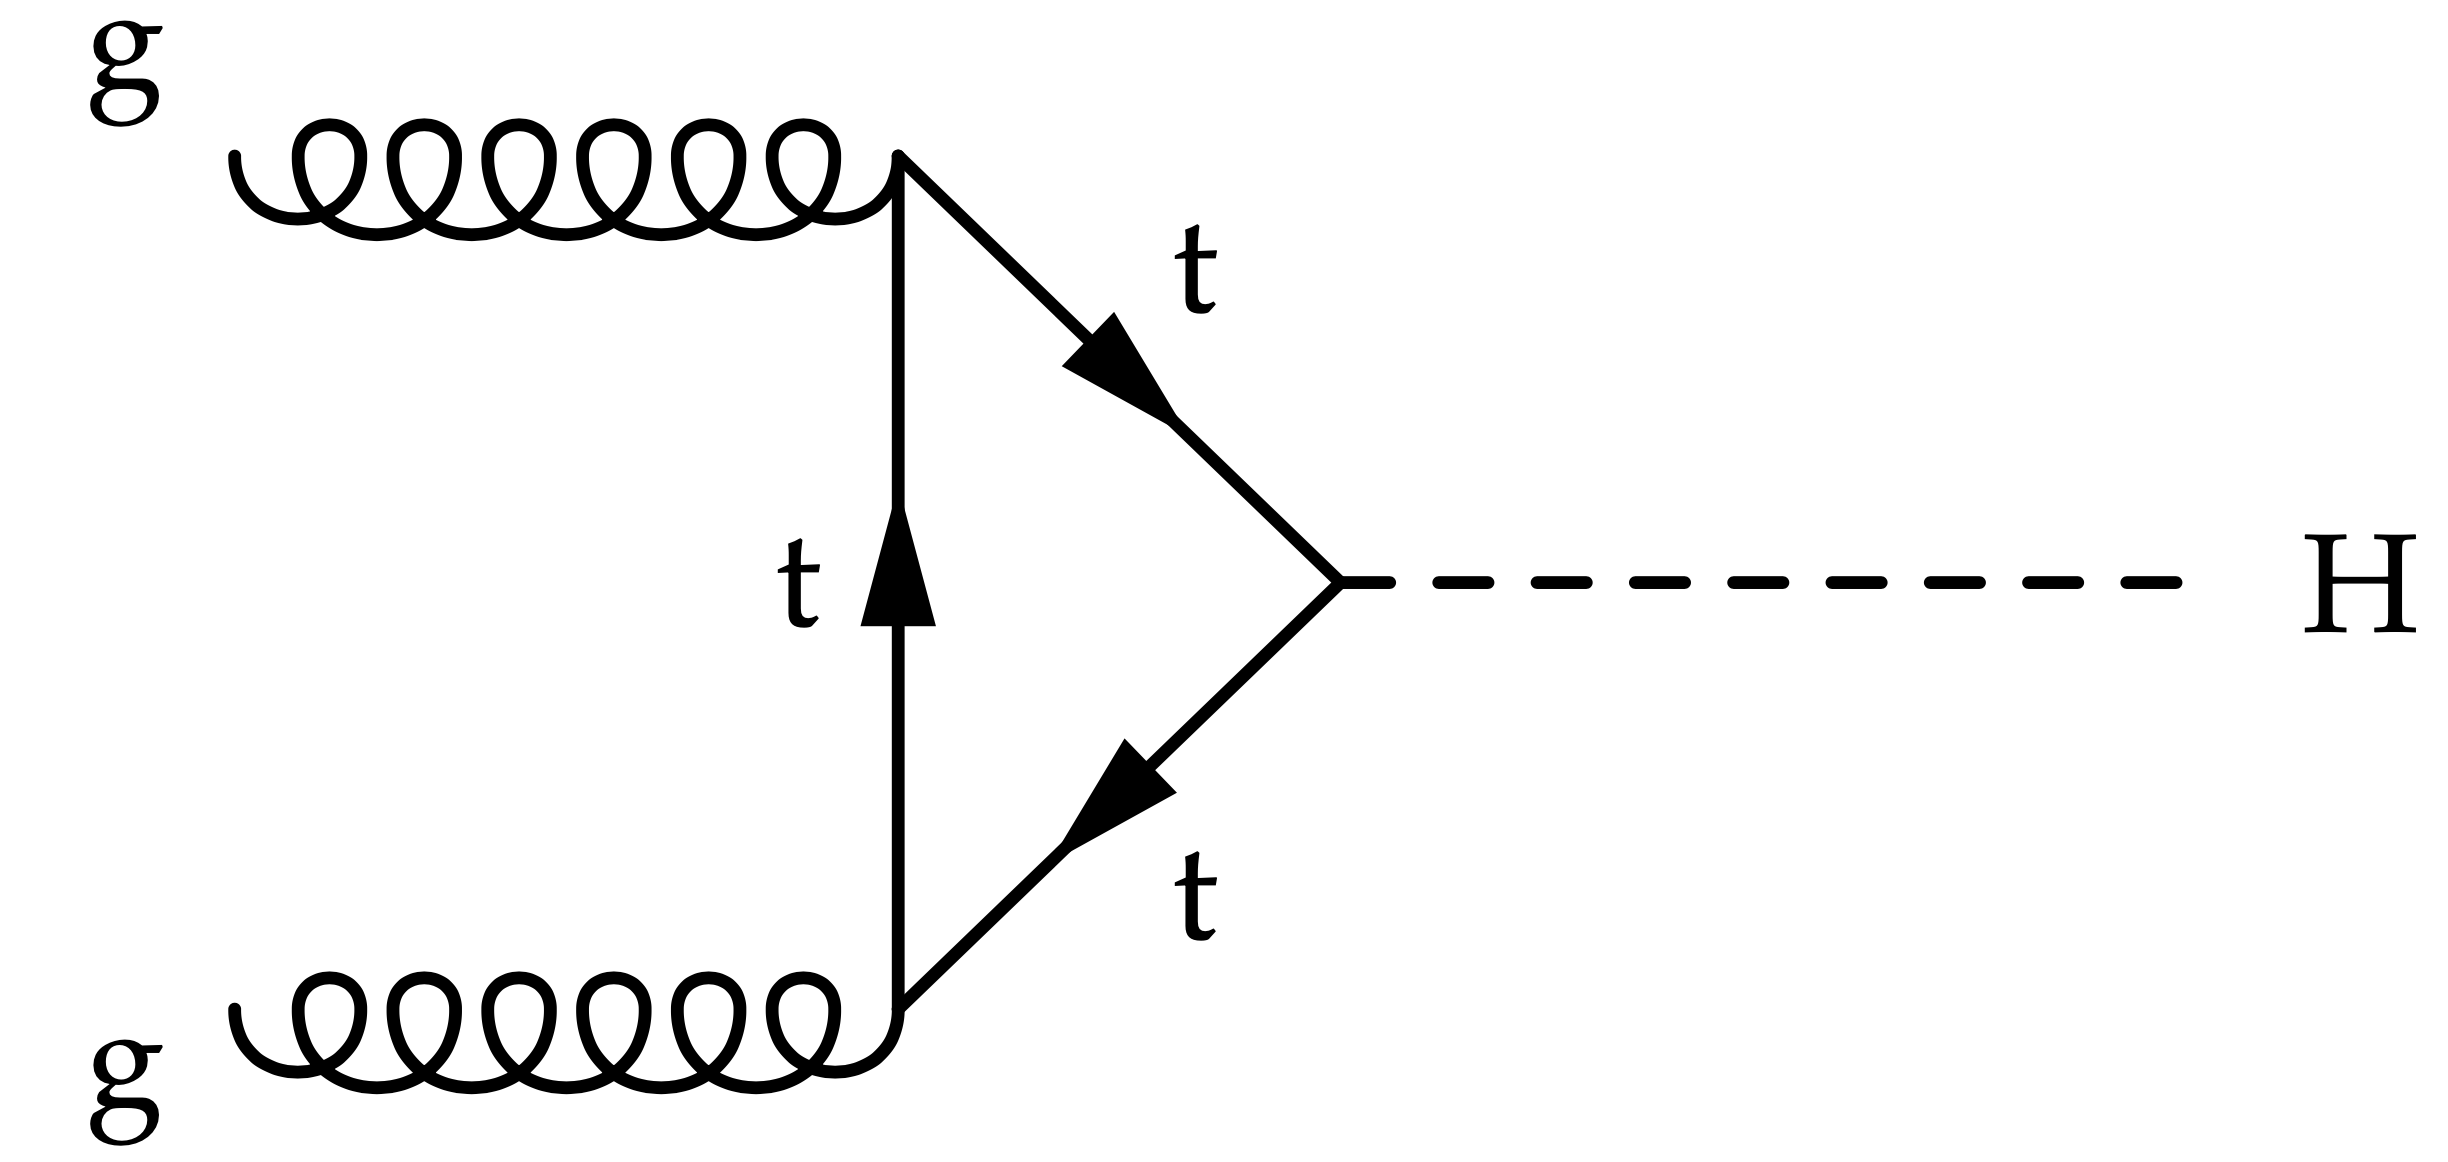
\includegraphics[width=\textwidth]{GGFH.png}
            \vspace{-0.5cm}
            \firstsubcaption{$ggF$}
            \label{GGFH}
        \end{subfigure}
        \hfill
        \begin{subfigure}[b]{0.475\textwidth}  
            \centering 
            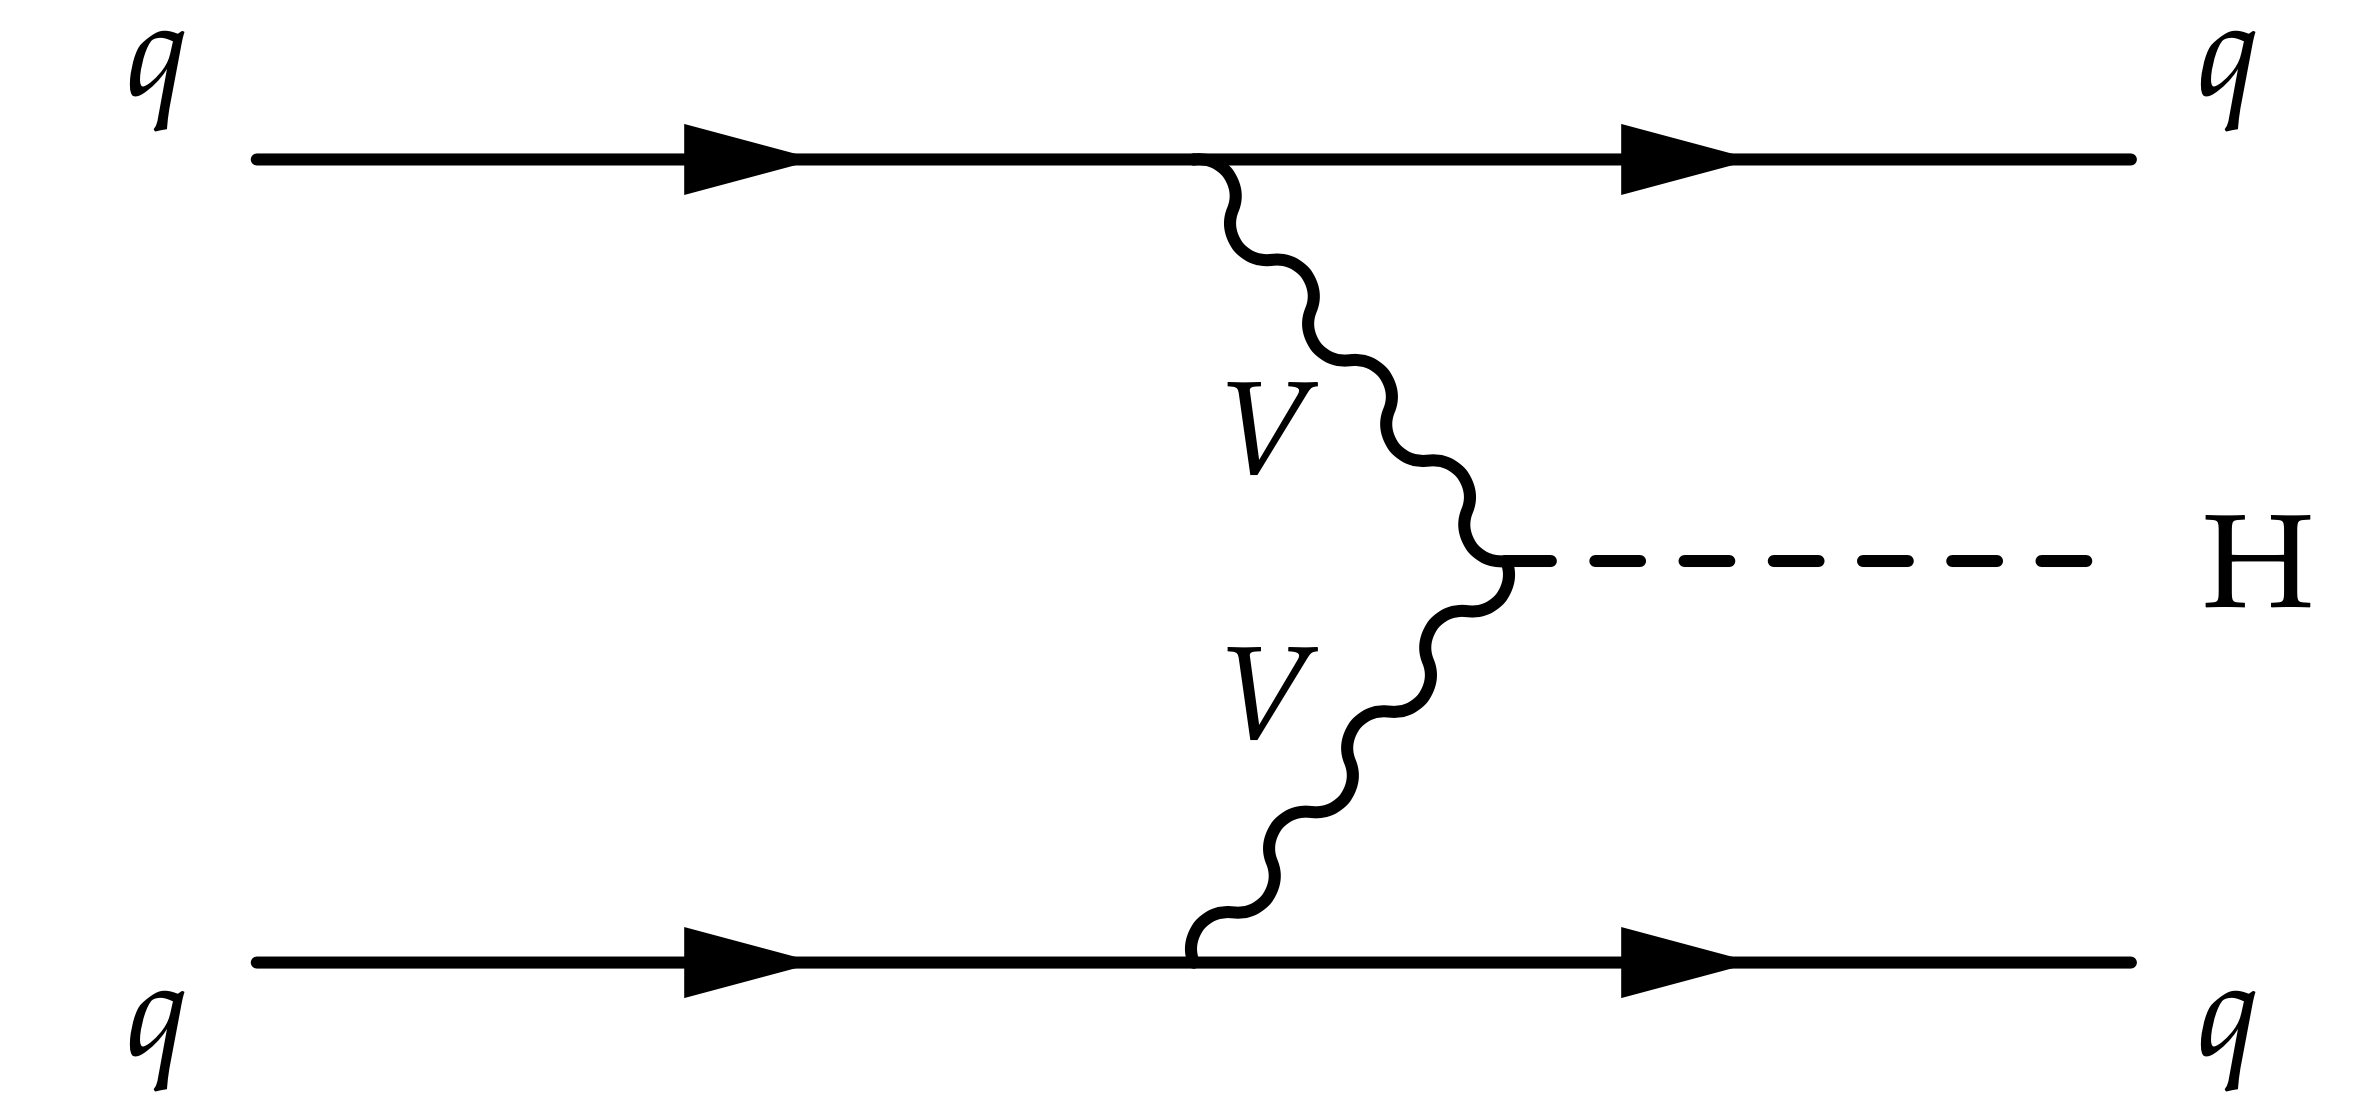
\includegraphics[width=\textwidth]{VBFH.png}
            \vspace{-0.5cm}
            \firstsubcaption{$VBF$}  
            \label{VBFH}
        \end{subfigure}
        \vskip\baselineskip
        \begin{subfigure}[b]{0.475\textwidth}   
            \centering 
            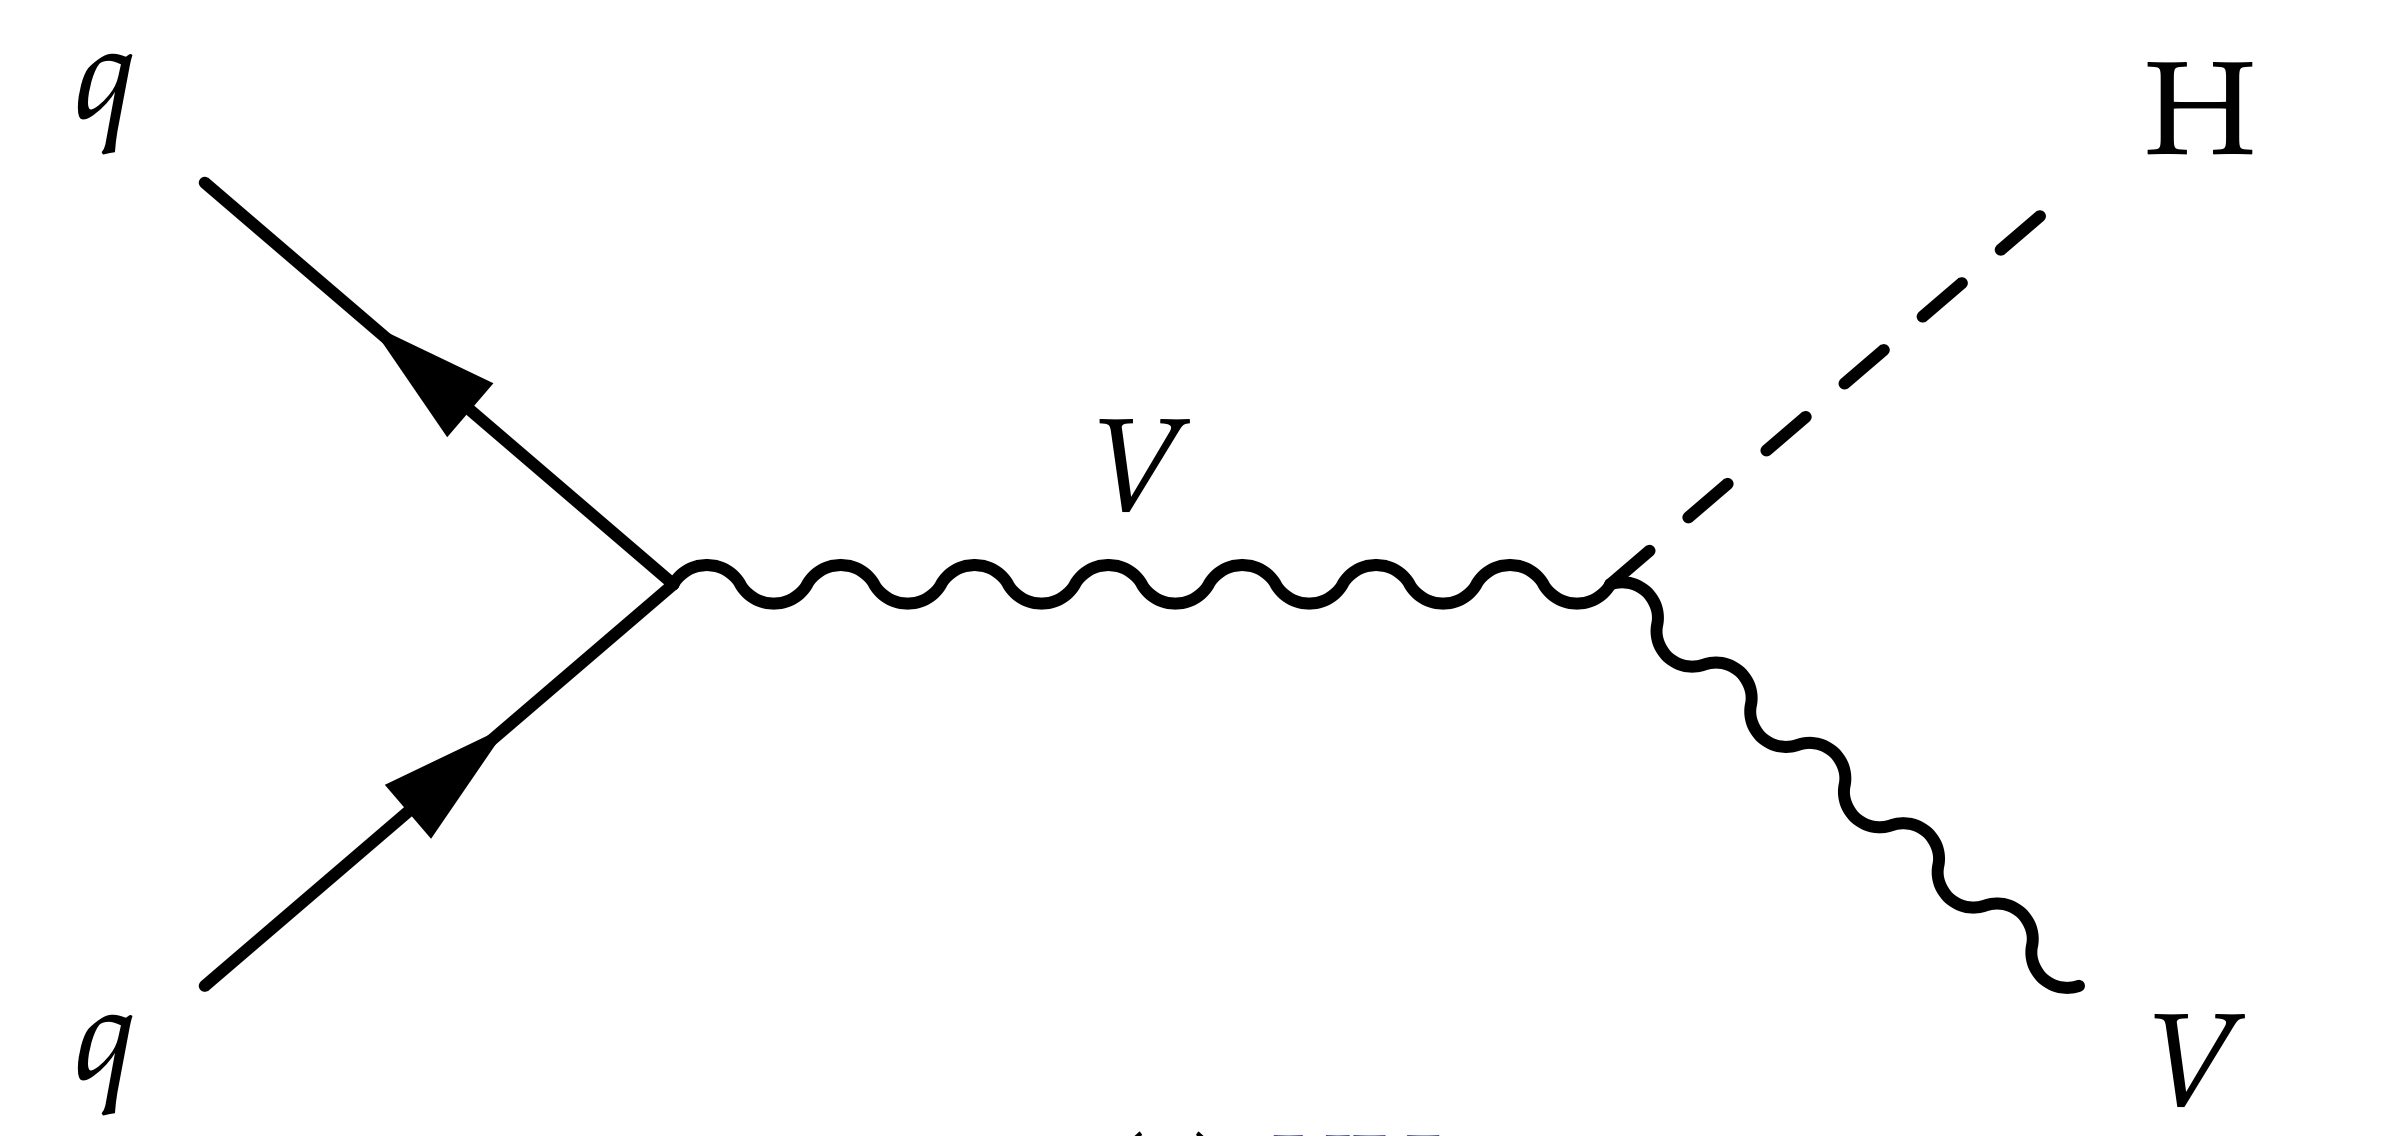
\includegraphics[width=\textwidth]{VH.png}
            \vspace{-0.5cm}
            \firstsubcaption{$VH$}    
            \label{VH}
        \end{subfigure}
        \hfill
        \begin{subfigure}[b]{0.475\textwidth}   
            \centering 
            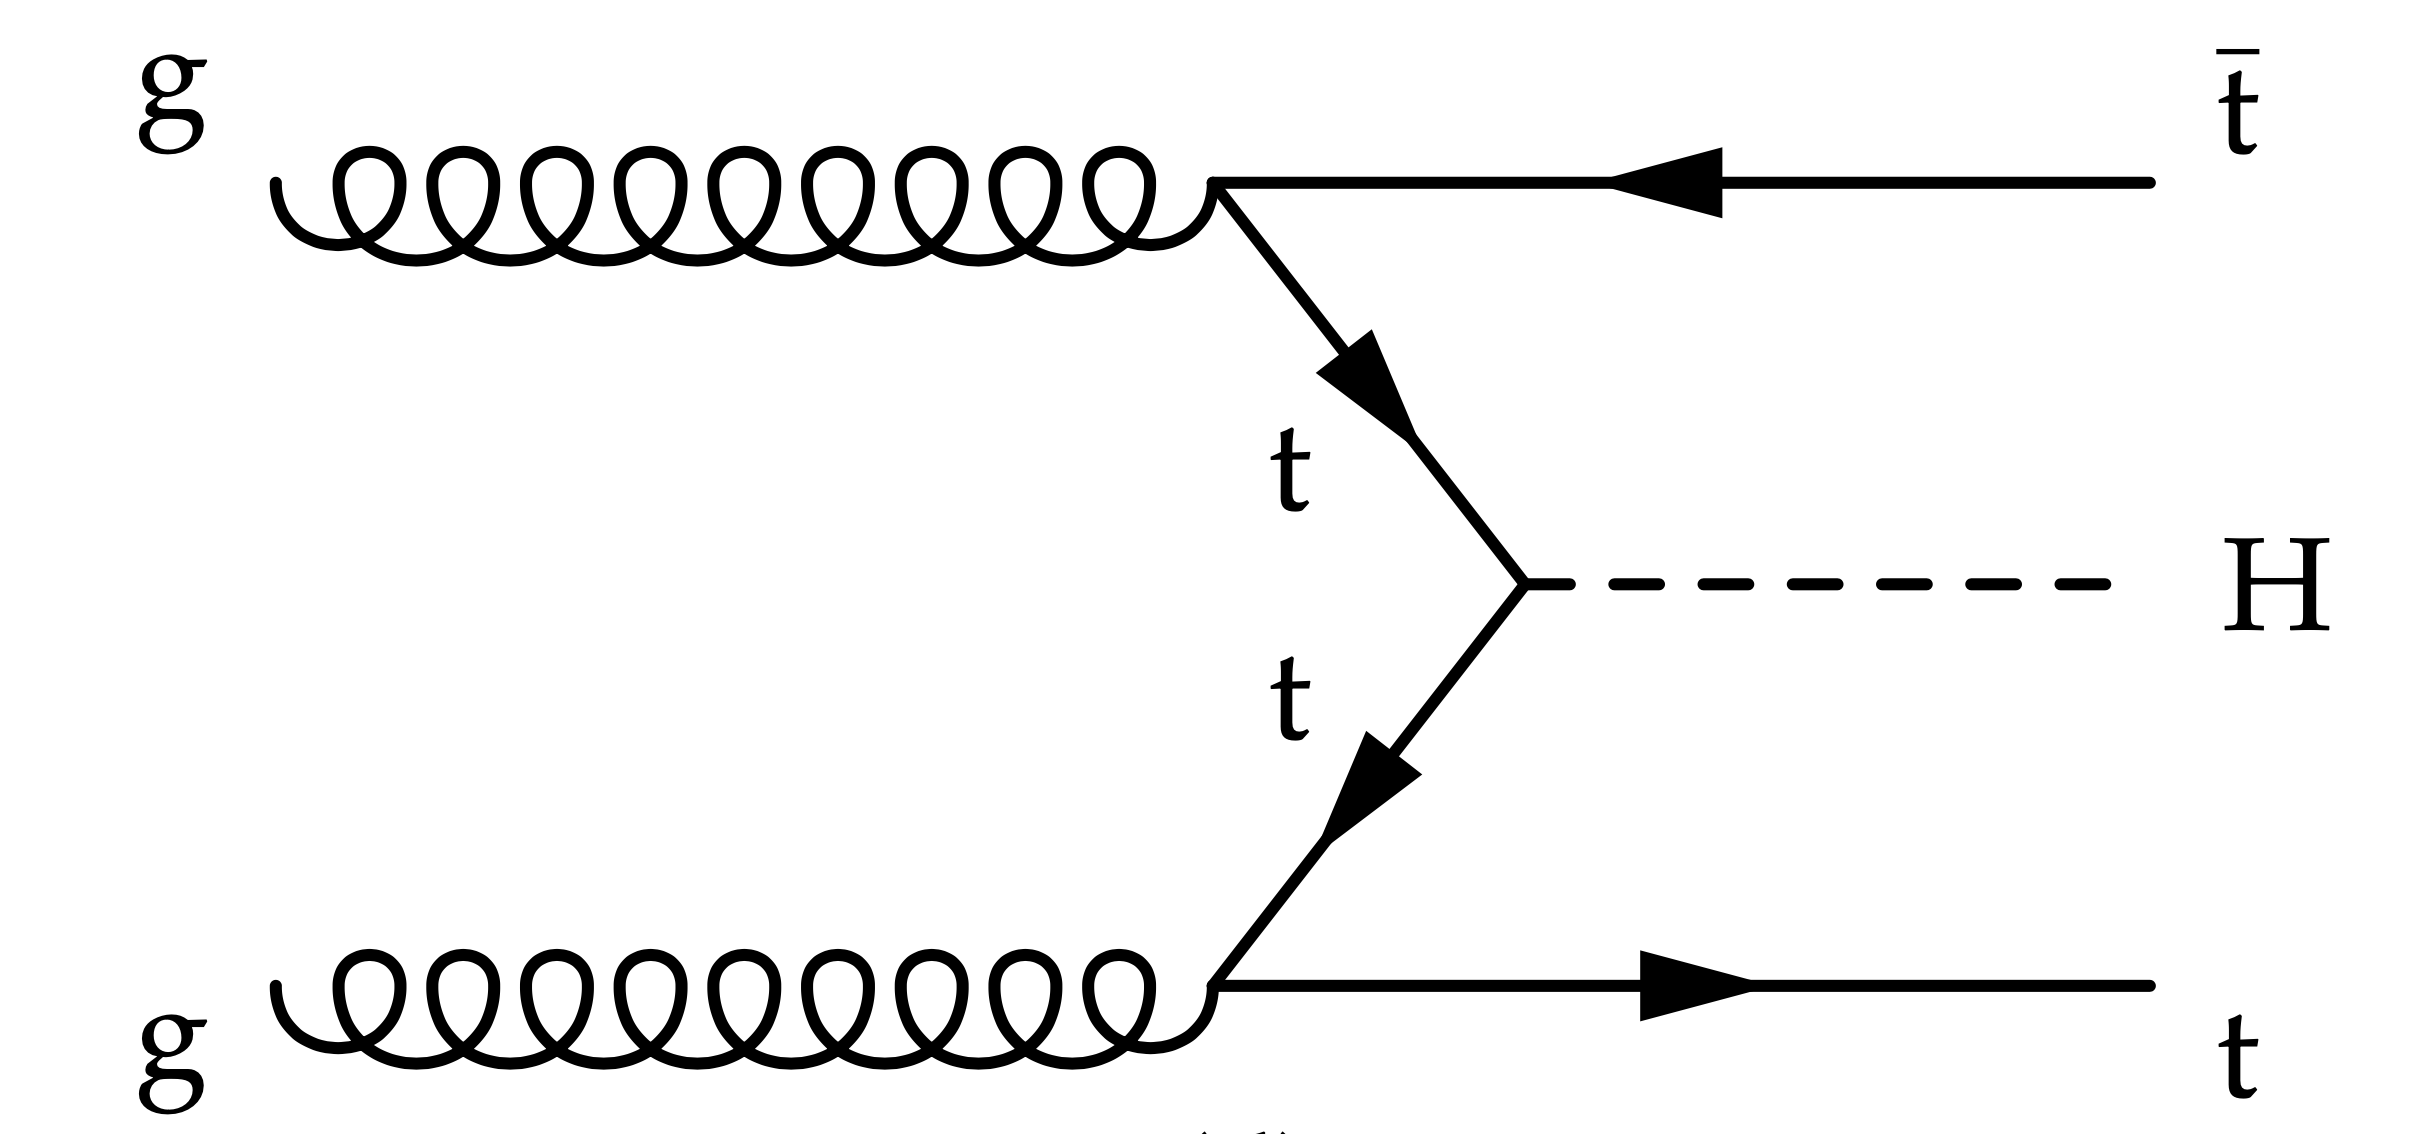
\includegraphics[width=\textwidth]{ttH.png}
            \vspace{-0.5cm}
            \firstsubcaption{$t\bar tH$}   
            \label{ttH}
        \end{subfigure}
        \caption[Feynman diagrams of Higgs boson productions at the LHC. The gluon fusion ($ggF$), vector boson fusion ($VBF$), Higgs strahlung ($VH$) and associated production with top quarks ($t\bar tH$) are shown. In the diagrams, $q$ denotes any quark, $t$ denotes the top quark, $V$ denotes any of the $Z$ or $W^\pm$ bosons.]
        {\small Feynman diagrams of Higgs boson productions at the LHC. The gluon fusion ($ggF$), vector boson fusion ($VBF$), Higgs strahlung ($VH$) and associated production with top quarks ($t\bar tH$) are shown. In the diagrams, $q$ denotes any quark, $t$ denotes the top quark, $V$ denotes any of the $Z$ or $W^\pm$ bosons.} 
        \label{HiggsFeynman}
    \end{figure*}

In the \textbf{\emph{gluon fusion production}} mode (ggF), shown at \autoref{GGFH}, two gluons produce a Higgs boson via a fermion loop but this fermion is usually the top quark since the Higgs boson couples to massive particles more often. This production mode has a cross section of 48.6 pb at $\sqrt{s} = 13$ TeV and is one order of magnitude larger than the second likely production mode at the proton-proton collisions. The Higgs boson produced in this mechanism is expected to have a small transverse momentum which can ease the event selection to separate the Higgs signal from background processes. 

The \textbf{\emph{vector boson fusion production}} mode (VBF) has a cross section of 3.78 pb at $\sqrt{s}=13$ TeV, whose Feynman diagram is shown in \autoref{VBFH}. This production mode scatters the quarks out of the protons and these quarks help characterising this production mode with two additional jets in the final state. This process can be observed in the particle detectors as two back-to-back jets that carry high transverse momentum at the forward regions.

WH and ZH associated production mechanism of the Higgs boson (VH), or the \textbf{\emph{Higgs strahlung}}, is the process of producing a $W^\pm$ or Z boson where a Higgs boson is radiated away. This production mode has a cross section of 2.25 pb at $\sqrt{s}=13$ TeV in pp collisions. The vector boson in the final state is a good signature for signal and background separation when decayed leptonically.

The fourth and final production mode is the \textbf{\emph{associated production with top quark pair}} ($t\bar tH$). This production mechanism is a rare process in pp collisions with a cross section of 0.5 pb at $\sqrt{s} = 13$ TeV. It is observed at the CMS Experiment in 2018 \cite{ttH-higgs}. The final state objects in this production mode, the top pair and the Higgs boson, can be identified by the large multiplicity of jets and leptons, however due to the lower cross section and the complex final state objects, this production mode is usually not included in the analyses and the same is valid for this thesis. When all of the standard model processes considered, the total cross section for the Higgs boson production makes it a rare process. The cross sections of the production modes of Higgs as a function of $\sqrt{s}$ is shown in \autoref{higgs-xsec-vs-sqrtS}.

\begin{figure*}[ht]
        \centering
        \begin{subfigure}[b]{0.475\textwidth}
            \centering
            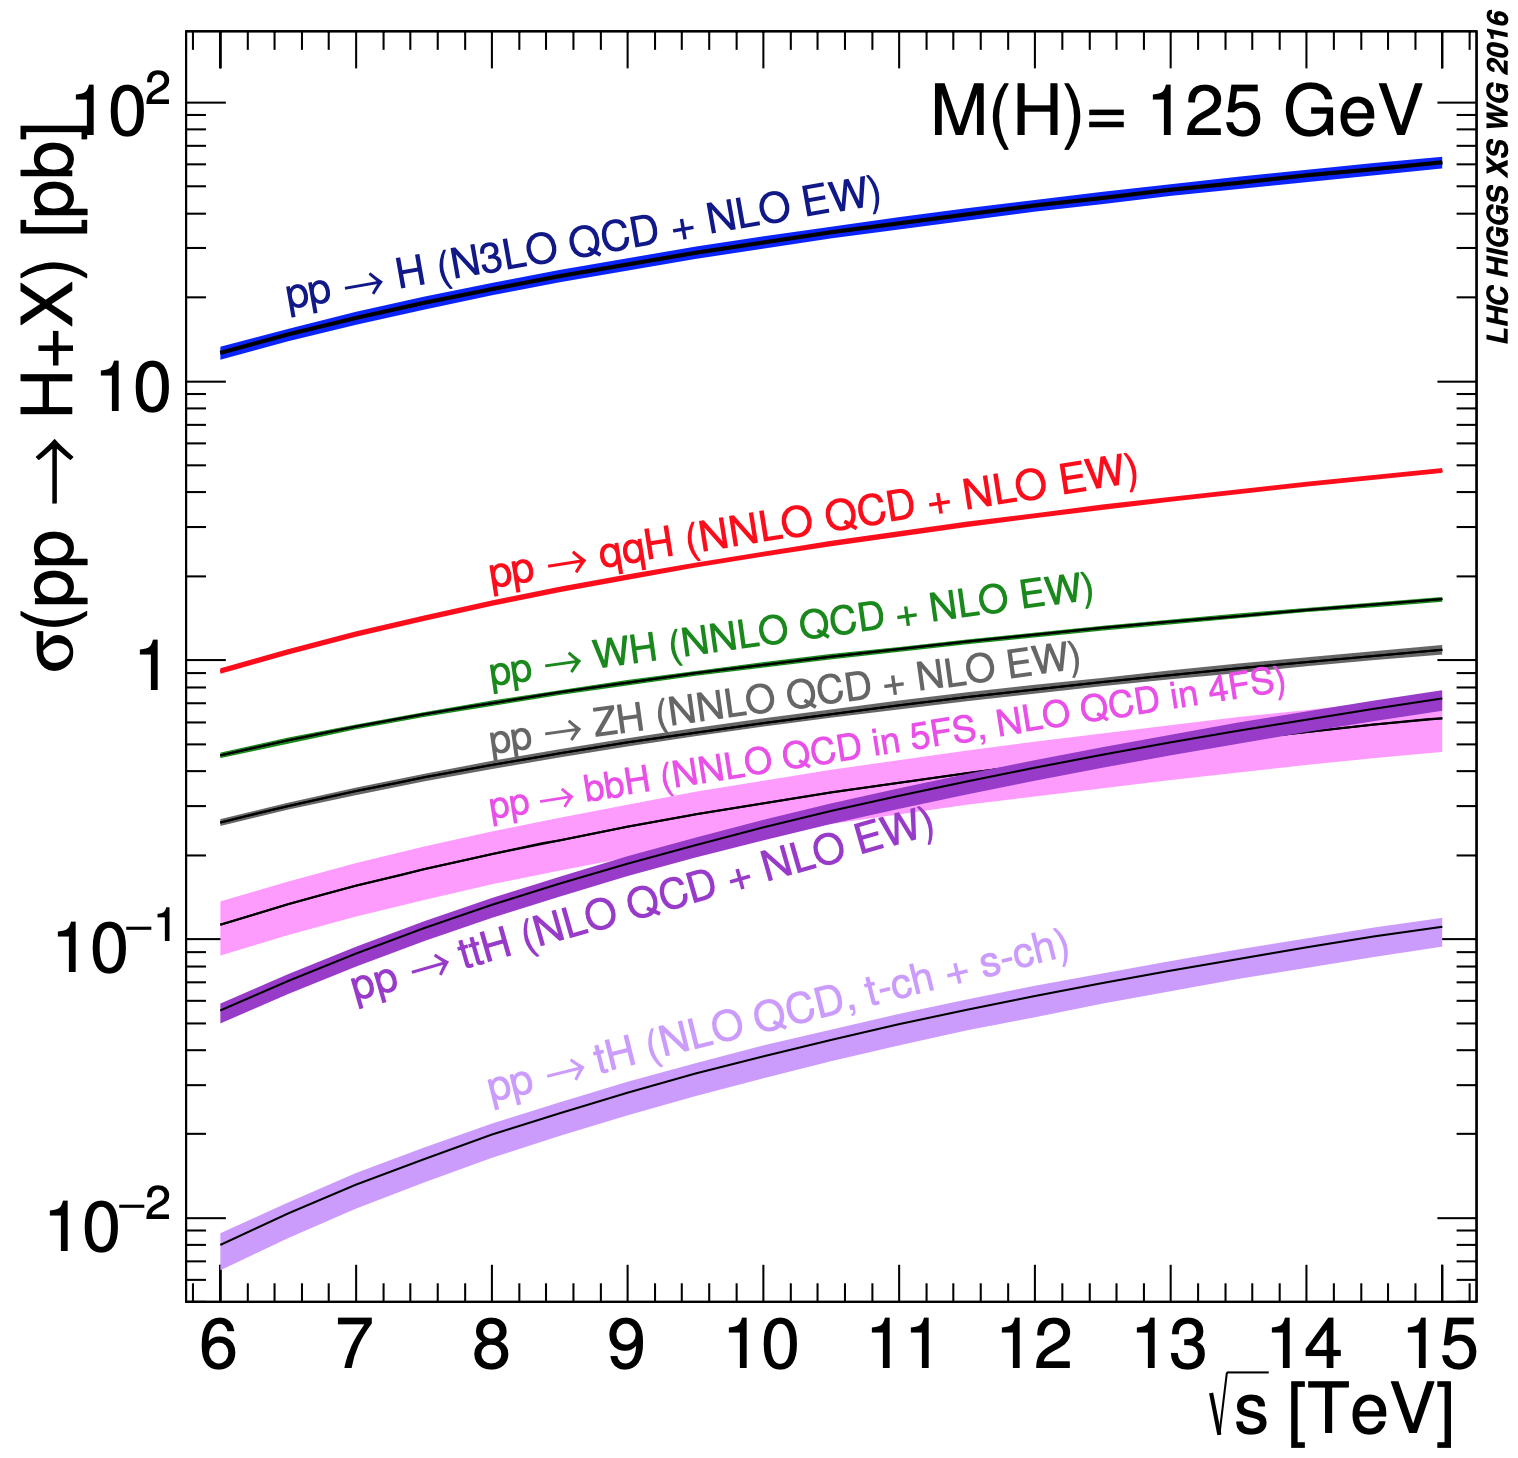
\includegraphics[width=\textwidth]{higgs-xsec-vs-sqrtS.png}
            \vspace{-0.75cm}
            \firstsubcaption{$\sigma_H$}
            \label{higgs-xsec-vs-sqrtS}
        \end{subfigure}
        \hspace{0.2cm}
        \begin{subfigure}[b]{0.475\textwidth}  
            \centering 
            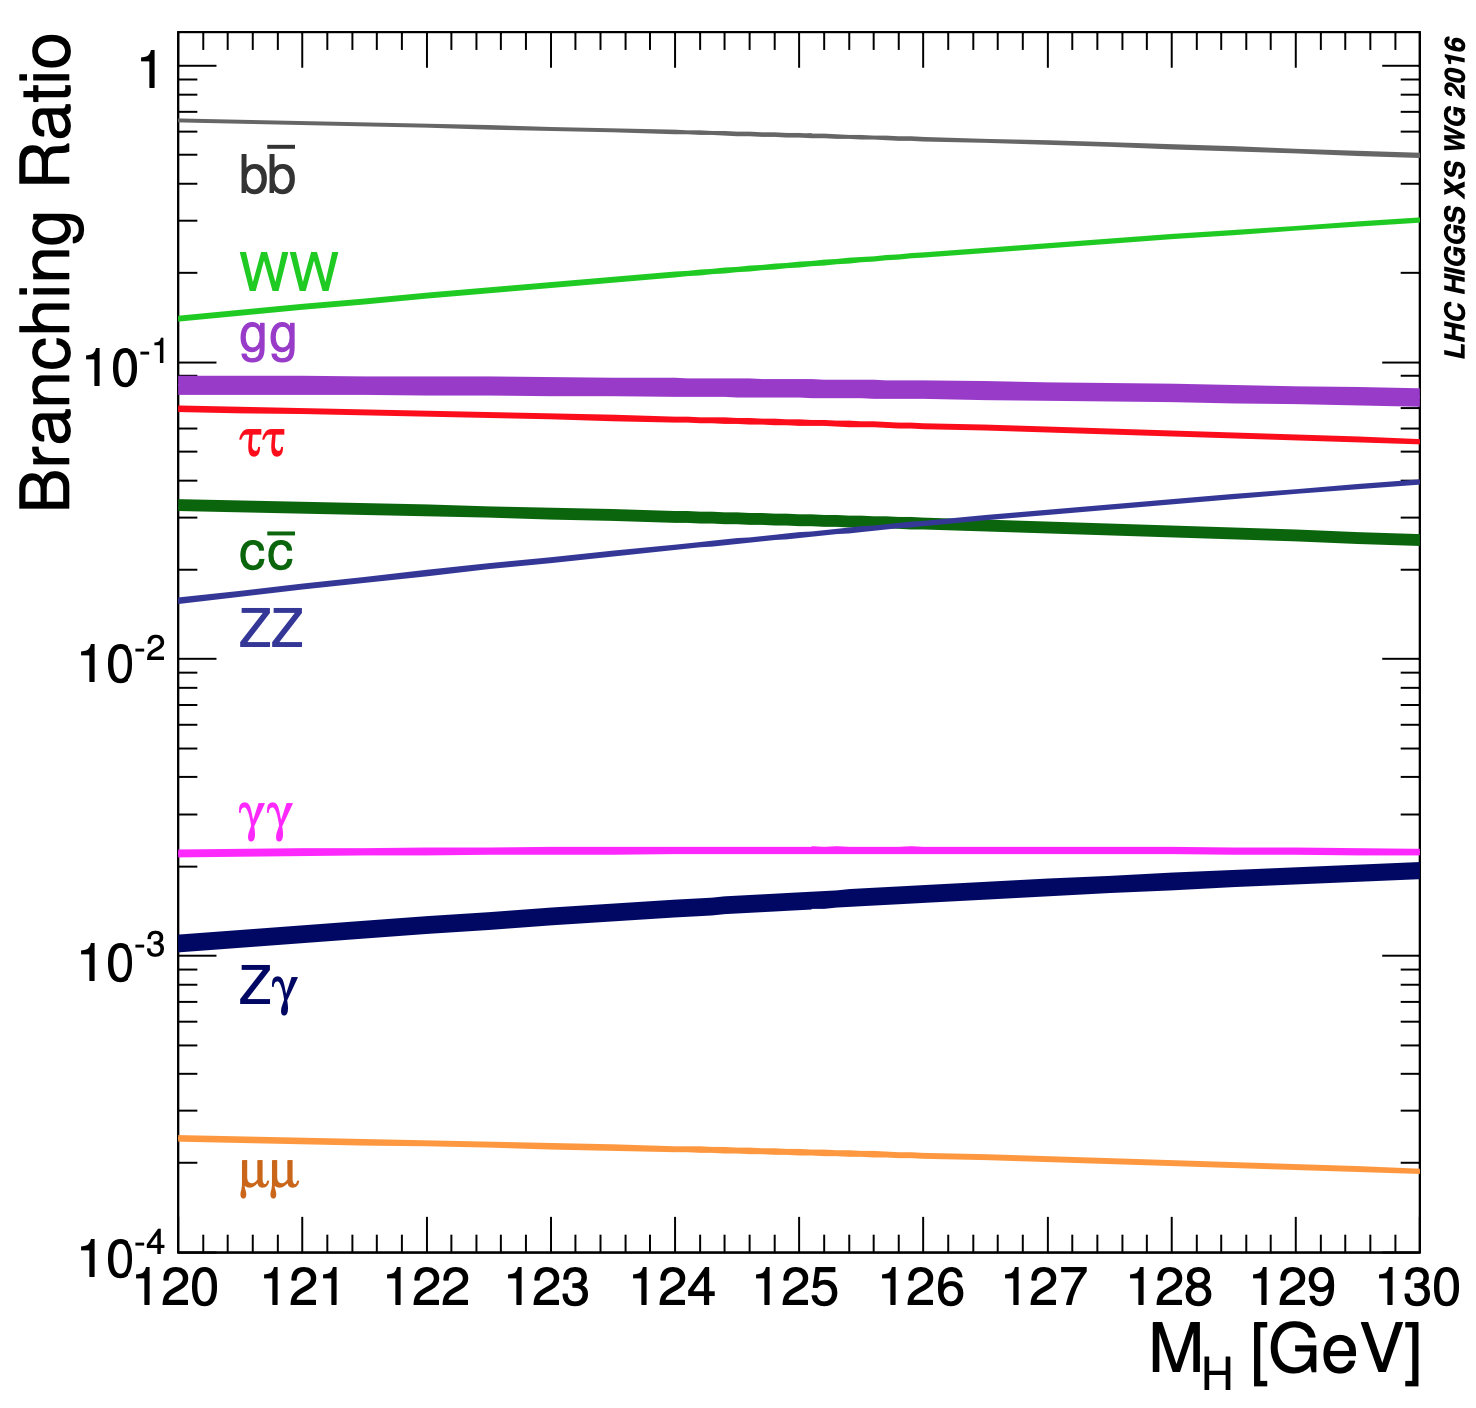
\includegraphics[width=\textwidth]{higgs-br-vs-mH.png}
            \vspace{-0.75cm}
            \firstsubcaption{$m_H$}
            \label{higgs-br-vs-mH}
        \end{subfigure}
        \caption[Higgs boson production cross section as a function of different production mechanisms (on the left). Branching fractions the Higgs boson as a function of $m_H$ .The theoretical uncertainties are indicated as bands in both plots.]
        {\small Higgs boson production cross section as a function of different production mechanisms\cite{higg-phen-3} (on the left). Branching fractions the Higgs boson as a function of $m_H$\cite{higgs-br-vs-mH}.The theoretical uncertainties are indicated as bands in both plots.}
\end{figure*}

The decay modes of the standard model Higgs boson around its mass region is shown in \autoref{higgs-br-vs-mH}, and branching ratios are given in \autoref{HiggsBRtable}. Since the decay channels of the Higgs is strictly dependent on its mass, the branching ratios vary too much, as can be seen in \autoref{higgs-br-vs-mH-complete}. At high Higgs masses, the decays into the $W^\pm$ and $Z$ bosons dominate the spectrum.  On the other hand, the decays in the lower mass region where $m_H \le 200\; GeV$ needs extensive searches since the decays become complicated. The decays in this region is dominated by the $b\bar b$ channel and the decay to $t\bar t$ is not observed since the top quark pair is too heavy. An interesting result is that the decays to $W^+W^-$ and to $ZZ$ channels have non-negligible branching ratios much below their masses. In such cases, one of the decay products is produced off-shell ($V^*$) while the other is expected to have its nominal mass. Regarding the decays to vector bosons, the $H\rightarrow 4l$ is often called \emph{\textbf{the golden channel}} because of the leptonic decay of the intermediate vector boson, where the background contribution from QCD interactions is highly reduced.

\begin{table*}[ht]
	{\setlength{\tabcolsep}{14pt}
		\caption[The branching ratios and the relative uncertainty for a SM Higgs boson with $m_H$ = 125 GeV.]{The branching ratios and the relative uncertainty for a SM Higgs boson with $m_H$ = 125 GeV\cite{higgs-br-vs-mH, higg-phen-3}.}
		\begin{center}
			\vspace{-6mm}
			\begin{tabular}{lcr}
				\hline \\[-2.45ex] \hline \\[-2.1ex]
				Decay channel & Branching ratio & Rel. Uncertainty \\
				\hline \\[-1.8ex]
                $H\rightarrow \gamma\gamma$ & $2.27x10^{-3}$ & $2.1\%$\\
                $H\rightarrow ZZ$ & $2.62x10^{-2}$ & $\pm 1.5\%$\\
                $H\rightarrow W^+W^-$ & $2.14x10^{-1}$ &$\pm 1.5\%$ \\
                $H\rightarrow \tau^+\tau^-$ & $6.27x10^{-2}$ &$\pm 1.6\%$ \\
                $H\rightarrow b\bar b$ & $5.82x10^{-1}$ & $^{+1.2\%}_{-1.3\%}$\\
                $H\rightarrow c \bar c$ & $2.89x10^{-2}$ &$^{+5.5\%}_{-2.0\%}$ \\
                $H\rightarrow Z\gamma$ & $1.53x10^{-3}$ & $\pm 5.8\%$\\
                $H\rightarrow \mu^+\mu^-$ & $2.18x10^{-4}$ &$\pm 1.7\%$ \\
				\hline
			\end{tabular}
			\vspace{-6mm}
		\end{center}
		\label{HiggsBRtable}}
\end{table*}

\begin{figure}[ht]
	\centering
	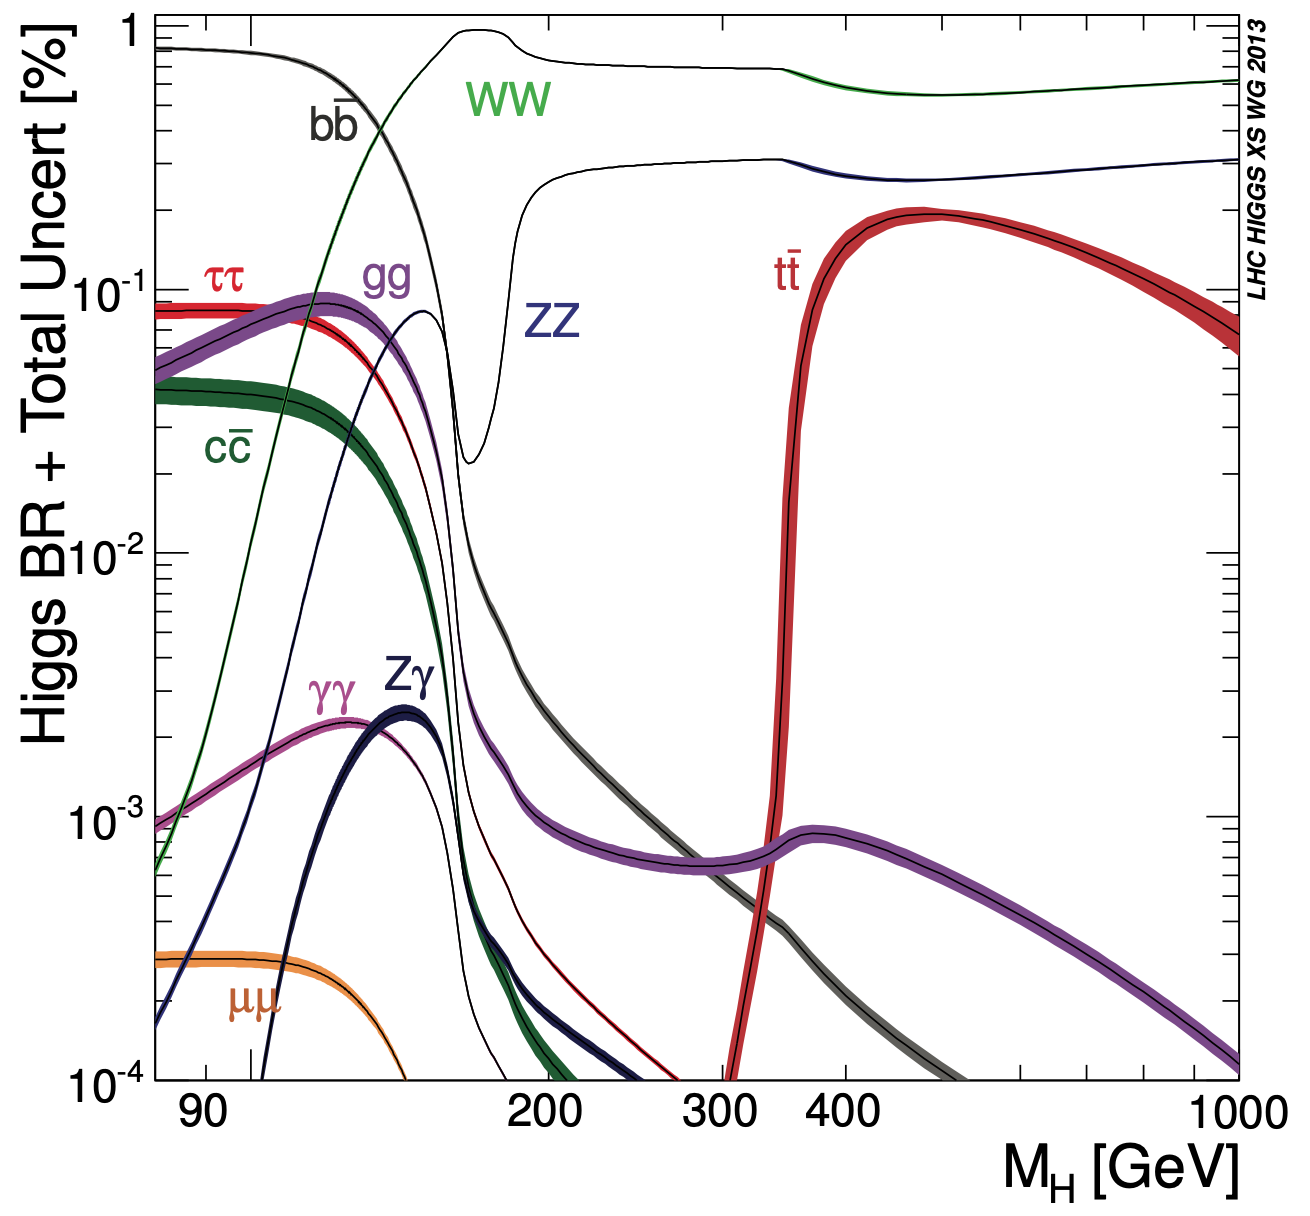
\includegraphics[width=\textwidth]{higgs-br-vs-mH-complete.png}
	\caption[Branching ratio of the Higgs boson decaying into various final states as a function of the Higgs boson mass.]{Branching ratio of the Higgs boson decaying into various final states as a function of the Higgs boson mass\cite{higg-phen-3}.}
	\label{higgs-br-vs-mH-complete}
\end{figure}


The diphoton decay of the Higgs boson occurs via a top quark or W boson loops. Although this decay channel is rare - its branching ratio is $2.27x10^{-3}$ -, it is a favourable decay mode since photons do not decay and can be reconstructed with a high accuracy in the detectors.

Another type of the decay modes of the Higgs boson is the leptonic decays; they have been first established in the $\tau^+\tau^-$ decay mode\cite{CMS-PAS-HIG-16-043}, further confirming the previous combined result from the ATLAS and CMS Experiments \cite{Aad2016}. In the recent years, the decay of the Higgs boson to a muon pair has been studied and an excess of events is observed in data corresponding to an integrated luminosity of $137 fb^{-1}$ with a significance of 3.0 standard deviations\cite{CMS-PAS-HIG-19-006}.

The tau pair decay of the Higgs boson, with a branching ratio of $6.27x10^{-2}$, can be observed in four production mechanisms that we have covered hence can have access to Yukawa couplings to fermions. Another importance of the $H\rightarrow\tau\bar\tau$ channel is to be the pioneering channel amongst the leptonic decays of the Higgs since the tau lepton is the heaviest of all known leptons. This feature of the $\tau\bar\tau$ channel may pave the way for any difference between the Higgs mechanisms to lepton and to quarks. Also, the final state particles of this decay mode have access to the Higgs properties such as spin and parity, but the reconstruction of the hadronic taus can be elaborate. 

\subsection{Higgs boson pair production}

The trilinear self-coupling of the Higgs boson was studied long before its discovery in 1988 \cite{GLOVER1988282}, emphasising that it can be measured from the Higgs boson pair production. There are other processes that contribute to the double Higgs boson production via different production mechanisms. The Higgs boson pairs are produced at the LHC by the similar mechanism as the Higgs boson productions. 

The \textbf{gluon fusion}, similar to the to the single Higgs gluon fusion production mechanism explained in \autoref{higgs-status}, starts with two gluons producing a Higgs boson via either i) a heavy quark loop, which finally produces a Higgs boson pair through the trilinear self-coupling (triangle type) or ii) two on-shell Higgs bosons emerge from the heavy quark loop (box type), as can be seen in \autoref{ggF-HH}. The relative contribution of these two processes can bee seen in \autoref{triangle-box-relative}. The cross section for this production mode is calculated up to next-to-next-to-leading order (NNLO) in QCD perturbation theory\cite{deFlorian2016}.

\begin{figure*}[ht]
        \centering
        \begin{subfigure}[b]{0.475\textwidth}
            \centering
            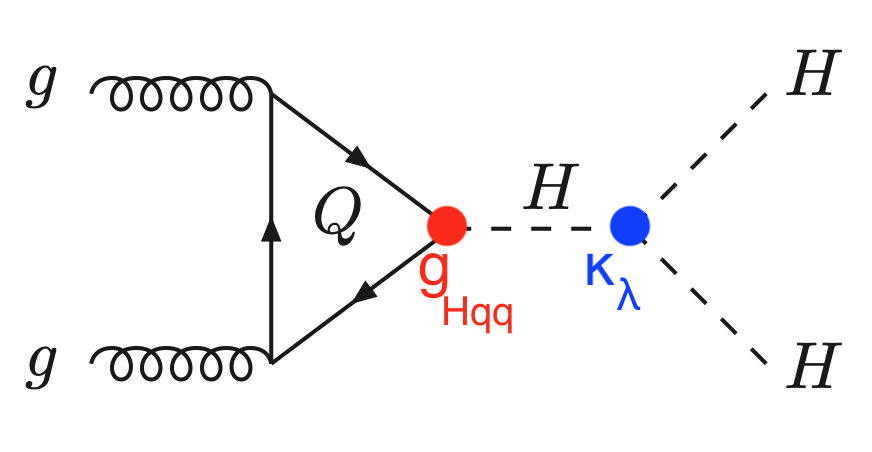
\includegraphics[width=\textwidth]{ggF1.png}
            \vspace{-0.5cm}
            \firstsubcaption{Triangle type}
        \end{subfigure}
        \hspace{0.2cm}
        \begin{subfigure}[b]{0.475\textwidth}  
            \centering 
            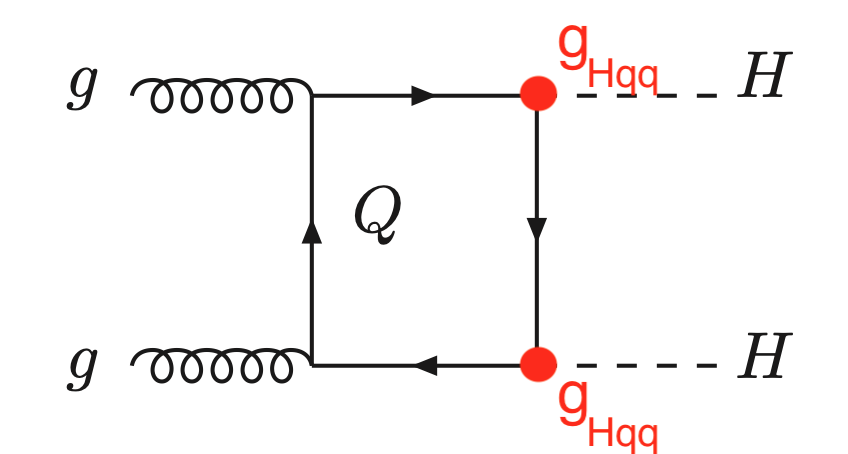
\includegraphics[width=\textwidth]{ggF2.png}
            \vspace{-0.5cm}
            \firstsubcaption{Box type}
        \end{subfigure}
        \caption[]
        {\small Feynman diagrams contributing at the leading order to Higgs boson pair production through (a) the self coupling of the Higgs boson and (b) through a top or bottom quark loop.}
        \label{ggF-HH}
\end{figure*}

\begin{figure}[ht]
	\centering
	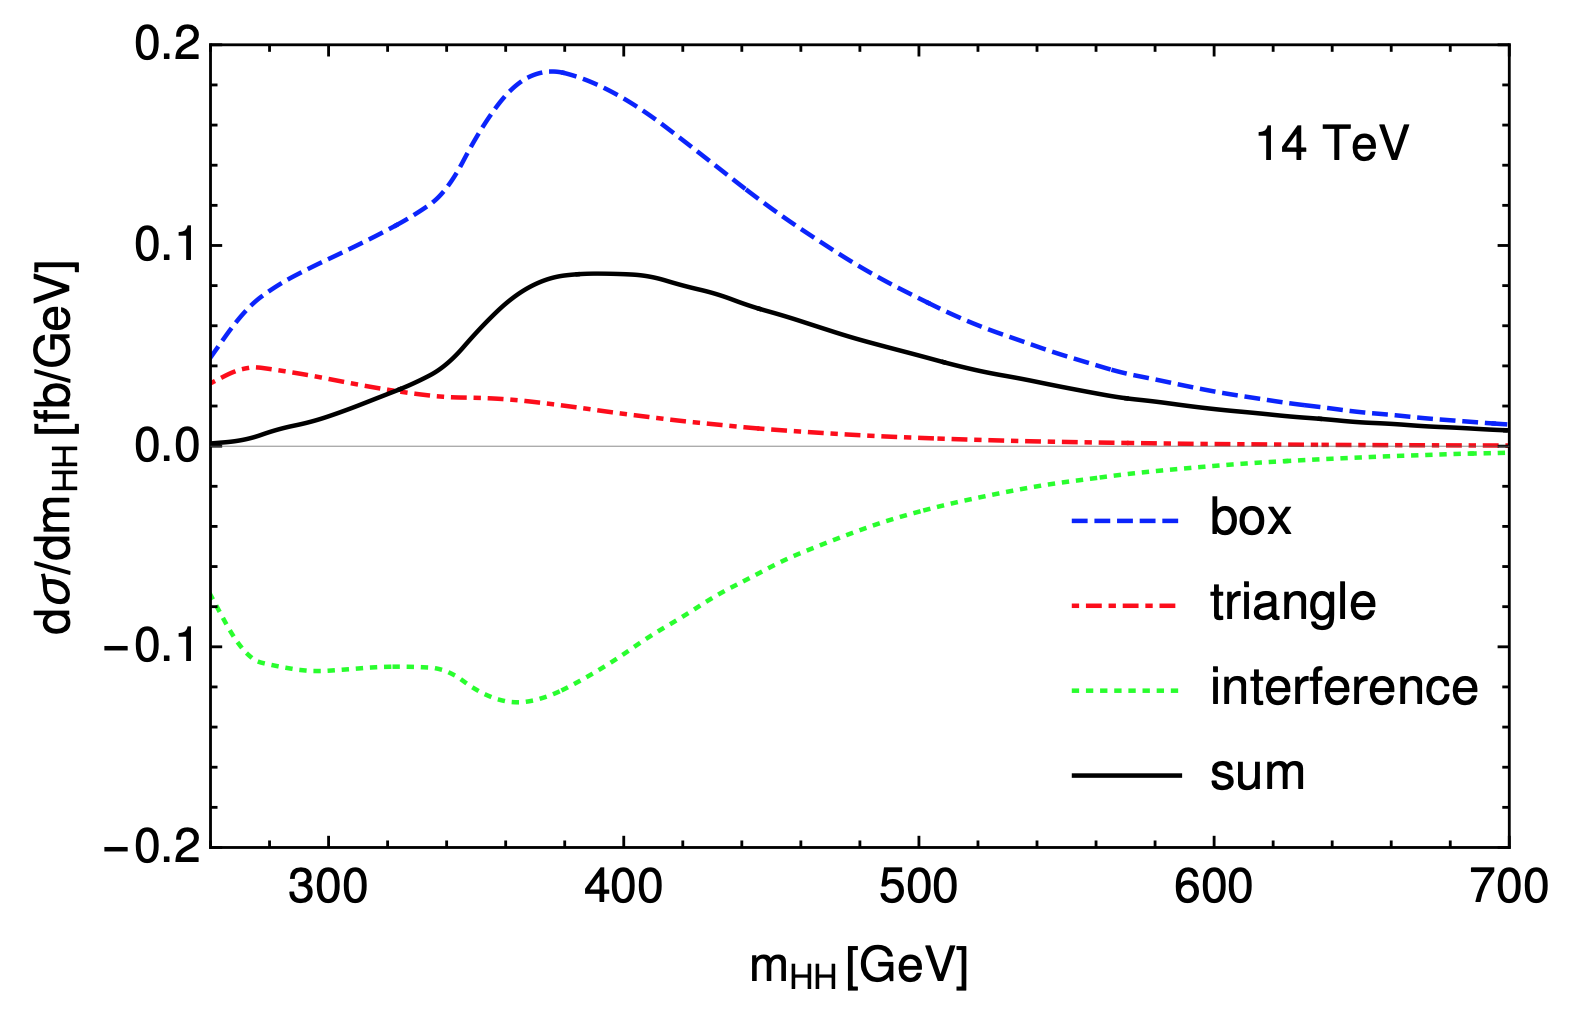
\includegraphics[width=\textwidth]{triangle-box-relative.png}
	\caption[Invariant mass distribution of Higgs boson pairs at leading order for the triangle and box-type gluon fusion production mechanism and their interference.]{Invariant mass distribution of Higgs boson pairs at leading order for the triangle and box-type gluon fusion production mechanism and their interference. The trilinear self-coupling reduces the cross section about a half w.r.t. the box-type process due to the large destructive interference\cite{DiMicco:2690841}.}
	\label{triangle-box-relative}
\end{figure}

The \textbf{vector boson fusion}, is the second production mechanism of double Higgs in terms of cross section. This production mechanism is dominated by t-channel W and Z boson exchange, similar to the single Higgs vector boson production mode. Three main Feynman diagrams contribute to this production; two Higgs radiations off the virtual W or Z boson shown in \autoref{vbfHH1} and \autoref{vbfHH2}, and a single off-shell Higgs boson splits into a Higgs pair \autoref{vbfHH3}. This production mechanism allows, in addition to the Higgs trilinear self-coupling, direct access to the Higgs boson coupling to a vector boson pair ($c_{2v}$) as well as to the Higgs boson coupling to two a single vector boson ($c_v$). Two back-to-back jets with high transverse momentum is the characteristic of this production mechanism analogous to the single Higgs vector boson fusion production. Other production mechanism of Higgs pair involve double Higgs strahlung, associated production with a top quark or a top quark pair, whose cross sections are very small. The cross sections of these production mechanisms at different centre-of-mass energies are given in \autoref{HHxsecTable} and as a function of the centre-of-mass-energy \autoref{HHxsecfigure}.

\begin{figure*}[ht]
        \centering
        \begin{subfigure}[b]{0.33\textwidth}
            \centering
            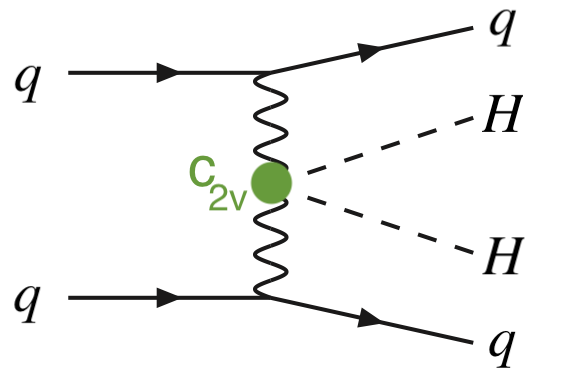
\includegraphics[width=\textwidth]{vbf1.png}
            \vspace{-0.5cm}
            \firstsubcaption{$c_{2v}$}
            \label{vbfHH1}
        \end{subfigure}
        \begin{subfigure}[b]{0.3\textwidth}  
            \centering 
            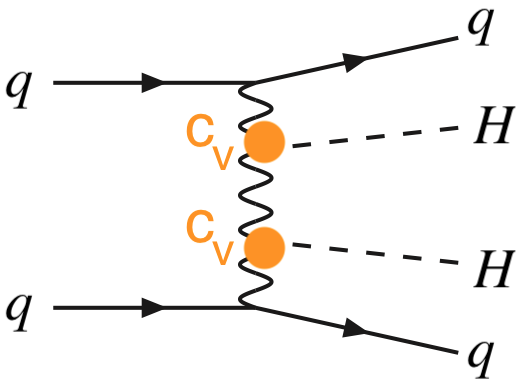
\includegraphics[width=\textwidth]{vbf2.png}
            \vspace{-0.5cm}
            \firstsubcaption{$c_{v}$}
            \label{vbfHH2}
        \end{subfigure}
        \begin{subfigure}[b]{0.35\textwidth}  
            \centering 
            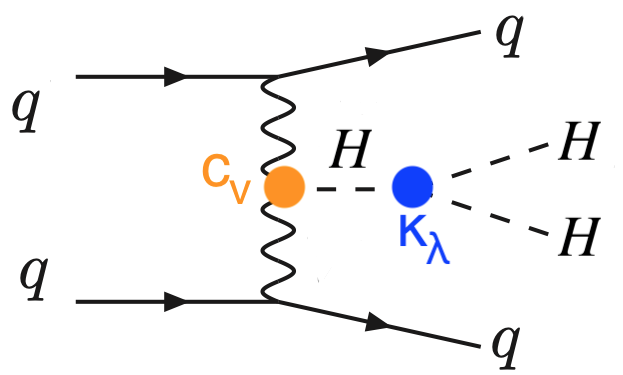
\includegraphics[width=\textwidth]{vbf3.png}
            \vspace{-0.5cm}
            \firstsubcaption{$\kappa_\lambda$}
            \label{vbfHH3}
        \end{subfigure}
        \caption[]
        {\small Feynman diagrams of the double Higgs boson production via vector boson fusion mechanism.}
\end{figure*}

\begin{table*}[ht]
	{\setlength{\tabcolsep}{14pt}
		\caption[Cross section (in pb) of the double Higgs boson production at different centre-of-mass ($\sqrt{s}$) energies for $m_H=125$ GeV. The theoretical uncertainties including the QCD factorisation and renormalisation scale ($\alpha_S$) uncertainties, Parton Distribution Function (PDF) uncertainty and effects from the top quark mass at NNLO can be found in the reference.]{Cross section (in pb) of the double Higgs boson production at different centre-of-mass ($\sqrt{s}$) energies for $m_H=125$ GeV. The theoretical uncertainties including the QCD factorisation and renormalisation scale ($\alpha_S$) uncertainties, Parton Distribution Function (PDF) uncertainty and effects from the top quark mass at NNLO can be found in \cite{higgs-br-vs-mH}.}
		\begin{center}
			\vspace{-6mm}
			\begin{tabular}{cccccc}
				\hline \\[-2.45ex] \hline \\[-2.1ex]
				$\sqrt{s}$ (TeV) &&&Production mode&&\\
				\hline \\[-1.8ex]
				& $ggF$ & $VBF$ & $t\bar tHH$ & $VHH$ & Total \\
				\hline \\[-1.8ex]
                8 & 10.15 & 0.459 & 0.174 & 0.355 & 11.14 \\
                13 & 33.49 & 1.62 & 0.772 & 0.864 & 36.74 \\
                14 & 39.59 & 1.95 & 0.949 & 0.979 & 44.47 \\
				\hline
			\end{tabular}
			\vspace{-6mm}
		\end{center}
		\label{HHxsecTable}}
\end{table*}

\begin{figure}[ht]
	\centering
	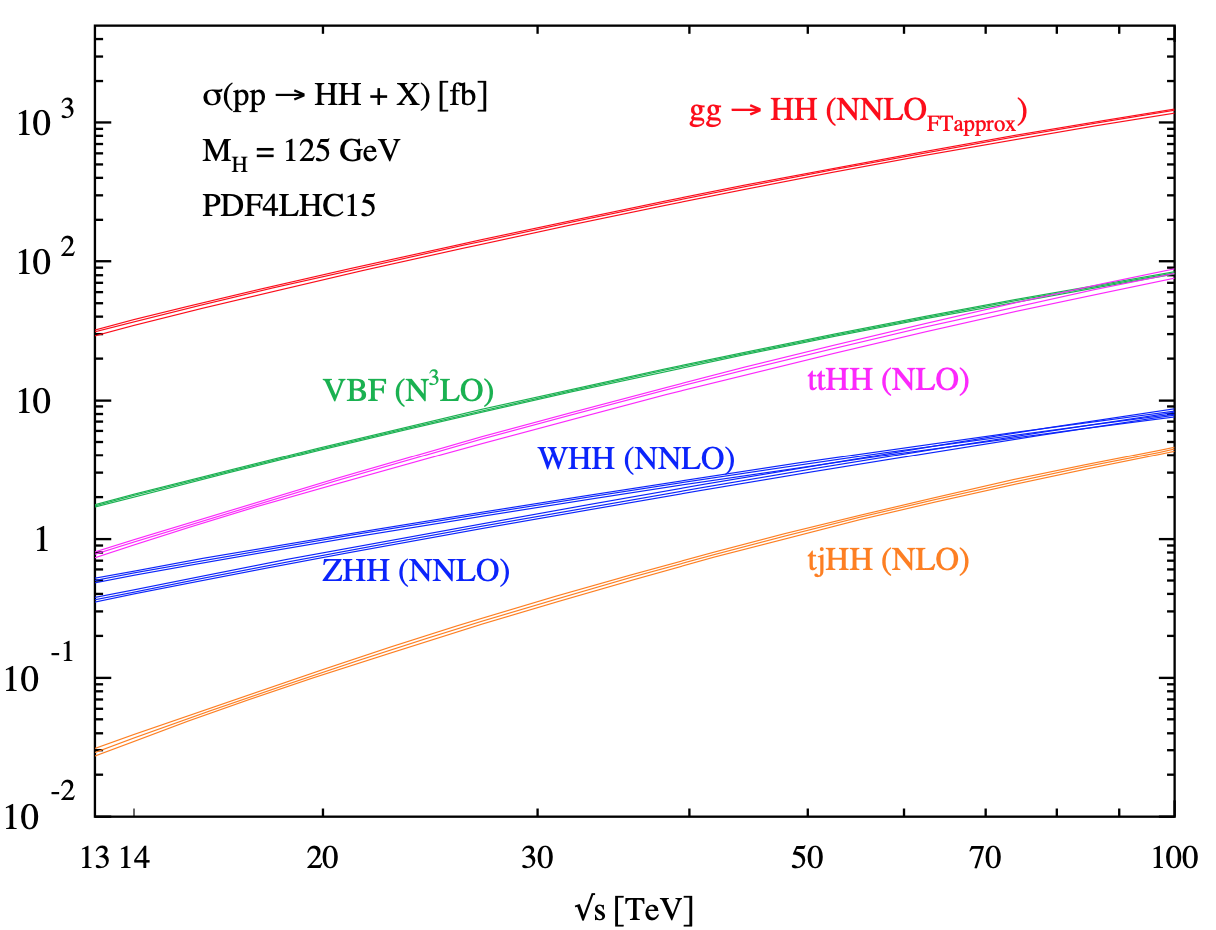
\includegraphics[scale=0.6]{HHxsecfigure.png}
	\vspace{2mm}
	\caption[Total cross section of double Higgs production mechanisms as a function of the centre-of-mass energy with $m_H = 125$ GeV within the SM. The gluon fusion remains the dominant production mode at high energies. The VBF continues to be the second dominant production mode while $t\bar tHH$ contribution starts to be in the order of VBF at about 100 TeV. The width of the lines shows indicate the total uncertainties coming from the scale and PDF + $\alpha_S$ uncertainties.]
	{Total cross section of double Higgs production mechanisms as a function of the centre-of-mass energy with $m_H = 125$ GeV within the SM. The gluon fusion remains the dominant production mode at high energies. The VBF continues to be the second dominant production mode while $t\bar tHH$ contribution starts to be in the order of VBF at about 100 TeV. The width of the lines shows indicate the total uncertainties coming from the scale and PDF + $\alpha_S$ uncertainties\cite{DiMicco:2690841}.}
	\label{HHxsecfigure}
\end{figure}

The double Higgs boson production is very rare at the LHC, hence the experimental searches include only the first two dominant production mechanism, as the same is valid for this thesis. As mentioned earlier, the latter allows the direct access to both the Higgs trilinear self-coupling and the Higgs coupling to vector bosons. The destructive interference of the vector boson fusion production along with the restricted phase space of the double Higgs, makes the double Higgs production very sensitive to BSM physics from which the contributions might require modifications to the theory which can be observed at the LHC data at hand. In this regards, the scans of $c_v$ and $c_{2v}$ couplings are aimed in this thesis as a test for the SM and a probe of BSM physics.

The SM expectations or the BSM models can be verified/rejected depending on the results of the decay mode searches of double Higgs production. The ATLAS and CMS Collaborations have discovered a rich variety of channels of double Higgs production. At Run I, these two collaborations have searched for both resonant and non-resonant productions in the following channels: $b\bar b\gamma\gamma$, $b\bar b\tau^+\tau^-$, $b\bar b\bar b$, $b\bar b4l$, $WW^*\gamma\gamma$, $\tau^+\tau^-\gamma\gamma$ and in some other final states \cite{pdg}. Most of these channel are updated in Run II by both ATLAS\cite{Aad2020} and CMS\cite{Sirunyan2019} Experiments.

The HH production processes are very rich in final states given the SM Higgs boson decays. The possible final states for HH processes are shown in \autoref{HHdecaymodes} by a simple combination calculation using branching ratios of single Higgs boson. Searches for double Higgs at the LHC focus on decay channels with large branching ratios since the HH production process itself has a rather small cross section at the pp colliders. A similar search is performed by the CMS experiment using Run II dataset and resulted in an upper limit as 22.2 times the SM cross section, shown in \autoref{HHupperlimit}. However other decay channels, such as $WW\gamma\gamma$, $WWWW$, $\tau\tau\tau\tau$, and $\tau\tau\gamma\gamma$ which is the main focus of this thesis, can be probed and is needed to set up a tighter upper limit on the cross section calculations using collision data to broaden our knowledge on the Higgs boson pair production. 

\begin{figure}[ht]
	\centering
	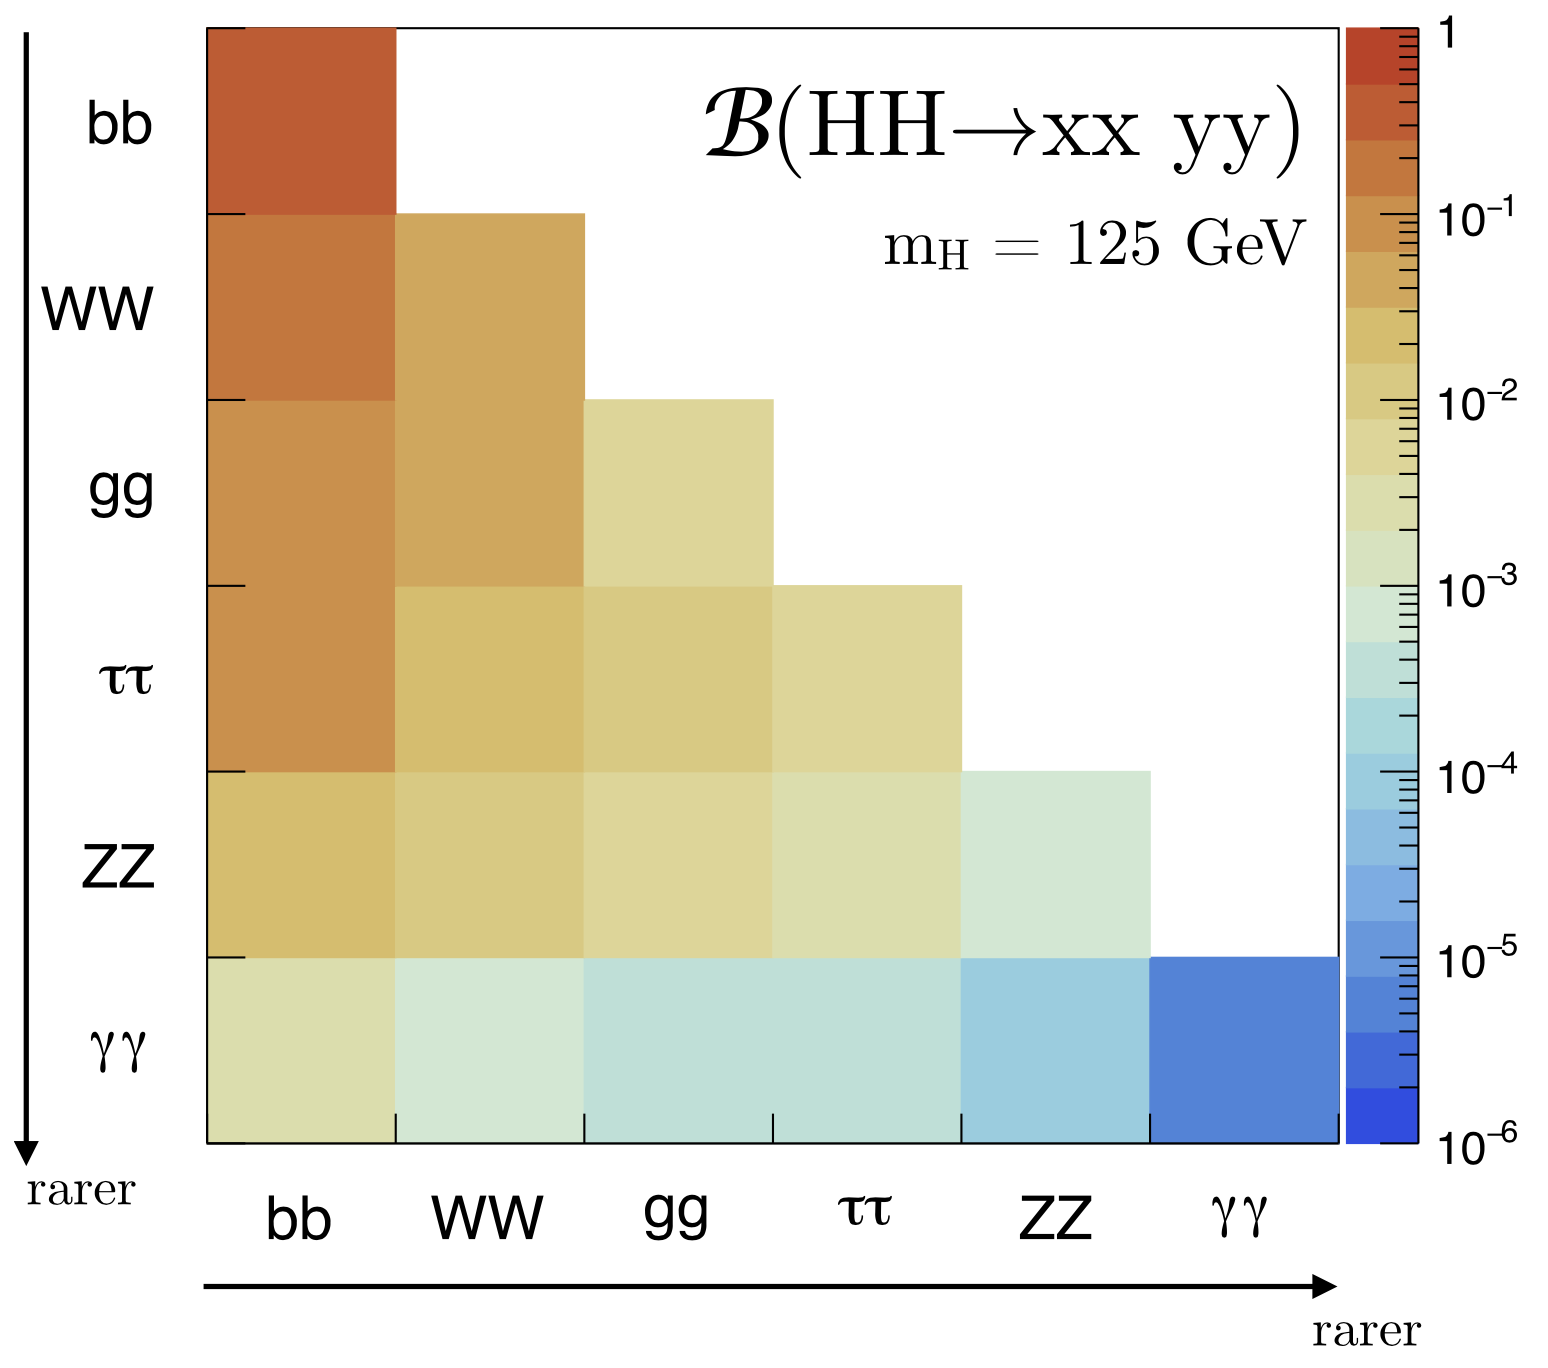
\includegraphics[scale=0.4]{HHdecaymodes.png}
	\vspace{2mm}
	\caption[Branching ratio of major double Higgs boson decay channels assuming a Standard Model Higgs boson. From top to bottom and left to right, less possible decay mode combinations are depicted. The logarithmic scale bar on the left indicates the branching ratio along with colours.]
	{Branching ratios of major double Higgs boson decay channels assuming a Standard Model Higgs boson\cite{Gouzevitch2020}. From top to bottom and left to right, less possible decay mode combinations are depicted. The logarithmic scale bar on the left indicates the branching ratio along with colours.}
	\label{HHdecaymodes}
\end{figure}

\begin{figure}[ht]
	\centering
	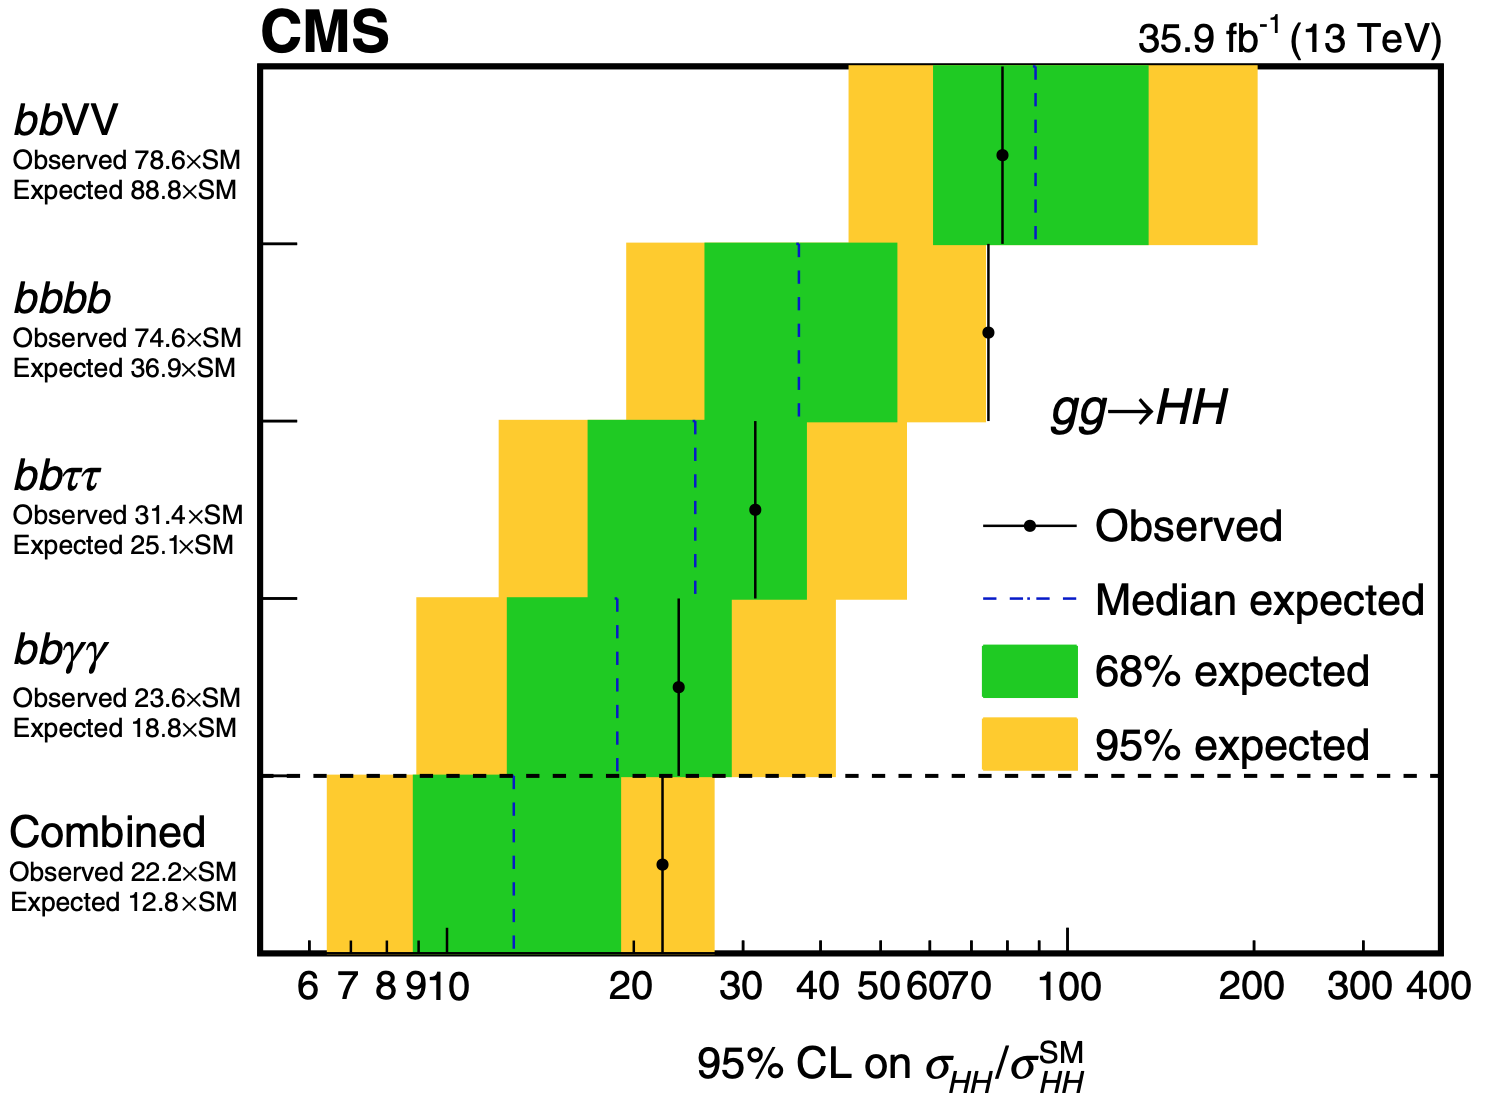
\includegraphics[scale=0.4]{HHupperlimit.png}
	\vspace{2mm}
	\caption[The 95\% CL upper limits on the signal strength $\mu = \sigma_{HH} / \sigma_{HH}^{SM}$ for $b\bar b$($VV/b\bar b/\tau^+\tau^-/\gamma\gamma$) channels along with with combined result. The inner green bands show 68\% and the outer yellow bands show the 95\% CL upper limits on $\mu$ under the background-only hypothesis.]
	{The 95\% CL upper limits on the signal strength $\mu = \sigma_{HH} / \sigma_{HH}^{SM}$ for $b\bar b$($VV/b\bar b/\tau^+\tau^-/\gamma\gamma$) channels along with with combined result. The inner green bands show 68\% and the outer yellow bands show the 95\% CL upper limits on $\mu$ under the background-only hypothesis\cite{Sirunyan2019}.}
	\label{HHupperlimit}
\end{figure}

% The searches regarding the self-coupling of the Higgs boson provided bounds on the $\kappa_\lambda$ parameter for the $b\bar b\gamma\gamma$ channel alone by ATLAS and CMS, such that,

% \be
% \begin{aligned}
% (ATLAS) -1.5 < \kappa_\lambda < 6.7 (observed), -2.4 < \kappa_\lambda < 7.7 (expected),\\
% (CMS) -3.3<\kappa_\lambda<8.5 (observed), -2.4<\kappa_\lambda<8.2(expected)
% \end{aligned}
% \ee
% where $\kappa_\lambda$ is the ratio between the Higgs trilinear coupling and its SM expectation.


\subsection{Beyond the Standard Model}

It is well known that the SM is one of the most successful theories in physics. However, the experiments show that there are some phenomena which the SM cannot explain. The main topics that are beyond the SM regarding the Higgs boson can be given in three main section.

The first phenomenon is the existence of three generations/families of fermions. The particles across the families are identical under many aspects however the Higgs couplings to them differ in several orders of magnitude and the SM is incapable of answering to this asymmetry. The second phenomenon is the mass of the Higgs boson itself, one of the free parameters of the SM shown in \autoref{SMparameters}. It is dependent on the radiative corrections and is not stabilised by any fundamental theory. Finally, the effectiveness of the theory up to the Planck scale can only be assured as far as the Higgs potential is bounded below for the vacuum to be stable. The stability of the potential at high energies is also associated with its conceivable role in the inflation theory of the Universe\cite{Bezrukov2008}. The model of Higgs as an inflation and the stability of the vacuum depend on the shape of the Higgs potential which is determined by the running self-coupling parameters $\lambda$. Therefore, it is reasonable to regard the SM as a manifestation of an unfolded embracing theory. The existence of the BSM physics could bring a solution to these problems.

Double Higgs boson production in this regard is a good handle to test our understanding of the Nature. If the new physics is at the energy scale of the LHC, new heavy states can be observed which then decay to a Higgs boson pair. This type of the production mechanisms is called the \textbf{\textit{resonant production}} and it shall manifest itself as an increase in the double Higgs cross section at a particular double Higgs boson invariant mass. The theories involving the existence of such particles are subject to modify the Higgs boson couplings. A considerable outcome is expected in such theories; the multiplet extension of the scalar Higgs field\cite{Dawson2017}, extra Higgs doublet models, namely Two-Higgs-Doublet Model (2HDM)\cite{Branco2012, BluscaMato2017}, and composite Higgs models \cite{Grber2011, contino2010tasi, JHEP08-2014-095}.

The \textbf{\textit{non-resonant production}} of Higgs pairs in the BSM models can contribute in the quantum loops in the Feynman diagrams for HH production hence can modify the kinematics of the process and increase the cross section, but without causing a resonance that decays to a Higgs boson pair, shown in \autoref{resonantHH}. 

%I WILL EXPAND THIS SECTION IF I INCLUDE THE KAPPA LAMBDA SCAN IN THE ANALYSIS. a good explanation is given in cappati thesis

\begin{figure}[ht]
	\centering
	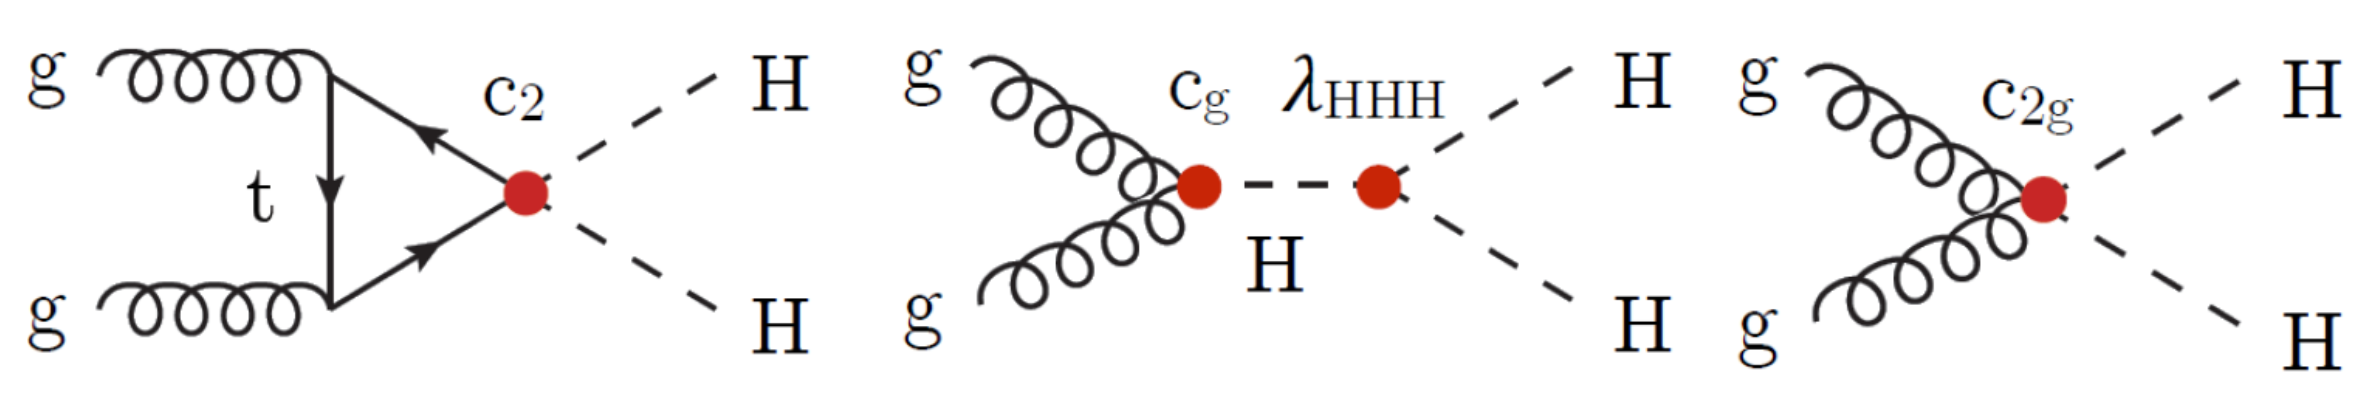
\includegraphics[width=\textwidth]{resonantHH.png}
	\vspace{2mm}
	\caption[Feynman diagrams that contribute to HH non-resonant production at LO with pure BSM effects.]
	{Feynman diagrams that contribute to HH non-resonant production at LO with pure BSM effects.}
	\label{resonantHH}
\end{figure}

% kappa framework

\newpage